%% Harbor Methodology Bench --- short report
%% Build:  tectonic -X compile brief.tex   (or: make brief)
%%
%% This is the focused version. The full 48-page treatment, with every table,
%% every censored trial, the complete correlation matrix and the full divergence
%% record, is main.tex / main.pdf.
\documentclass[11pt,a4paper]{article}

\usepackage[T1]{fontenc}
\usepackage{newtxtext,newtxmath}
\usepackage[a4paper,margin=2.4cm,bottom=2.8cm]{geometry}
\usepackage{graphicx}
\usepackage{booktabs}
\usepackage{multirow}
\usepackage{array}
\usepackage{xcolor}
\usepackage{amsmath}
\usepackage[labelfont=bf,font=small,justification=raggedright,singlelinecheck=false]{caption}
\usepackage{enumitem}
\usepackage{microtype}
\usepackage{fancyhdr}
\usepackage{titlesec}
\usepackage[round]{natbib}
\usepackage[hidelinks]{hyperref}

\definecolor{accent}{HTML}{2A78D6}
\definecolor{warn}{HTML}{EB6834}
\definecolor{good}{HTML}{1BAF7A}
\definecolor{shade}{HTML}{F5F5F2}

\hypersetup{colorlinks=true,linkcolor=accent,citecolor=accent,urlcolor=accent}
\setlist[itemize]{leftmargin=1.3em,itemsep=0.15em,topsep=0.3em}
\setlist[enumerate]{leftmargin=1.6em,itemsep=0.15em,topsep=0.3em}
\renewcommand{\arraystretch}{1.12}
\setlength{\tabcolsep}{5pt}
\titleformat{\section}{\normalfont\large\bfseries}{\thesection}{0.7em}{}
\titleformat{\subsection}{\normalfont\normalsize\bfseries}{\thesubsection}{0.6em}{}

\pagestyle{fancy}
\fancyhf{}
\fancyhead[L]{\small\color{black!55}The cost of process --- short report}
\fancyhead[R]{\small\color{black!55}\thepage}
\renewcommand{\headrulewidth}{0.4pt}
\setlength{\emergencystretch}{2.5em}
\sloppy

\newsavebox{\findingbox}
\newenvironment{finding}[1]
  {\par\medskip\noindent\begin{lrbox}{\findingbox}%
   \begin{minipage}{\dimexpr\linewidth-2\fboxsep-4pt}%
   \vspace{3pt}\textbf{\color{accent}#1}\par\smallskip\small}
  {\vspace{4pt}\end{minipage}\end{lrbox}%
   \noindent\textcolor{accent}{\vrule width 2pt height \dimexpr\ht\findingbox\relax depth \dimexpr\dp\findingbox\relax}%
   \colorbox{shade}{\usebox{\findingbox}}\par\medskip}

\newcommand{\code}[1]{\texttt{\small #1}}
\newcommand{\task}[1]{\texttt{\footnotesize #1}}

\begin{document}

\thispagestyle{empty}
\noindent{\color{accent}\rule{\linewidth}{1.2pt}}\par\vspace{0.35cm}
{\LARGE\bfseries The Cost of Process\par}
\vspace{0.25cm}
{\large What a repository's agent configuration actually buys a coding agent\par}
\vspace{0.3cm}
{\normalsize 156 trials, 26 Terminal-Bench 2.0 tasks, two opposite task populations, \$201.37\par}
\vspace{0.3cm}
\noindent{\color{accent}\rule{\linewidth}{1.2pt}}\par\vspace{0.45cm}

\noindent
{\small Christoph Mitschka \quad$\cdot$\quad
\href{mailto:christoph.mitschka@korza.ai}{christoph.mitschka@korza.ai} \quad$\cdot$\quad \today\\[0.15cm]
With an independent critical review contributed by \textbf{Antigravity} (Google DeepMind).
Short report; the full treatment is \code{main.pdf}.}

\vspace{0.45cm}
\hrule
\vspace{0.35cm}

\noindent\textbf{\large Summary}
\smallskip

\noindent Two published coding-agent toolkits --- \textbf{CodeZen} (delegation and review)
and \textbf{SDD} (a seven-step specification chain) --- were frozen at a Git SHA, injected as
a Docker layer into Terminal-Bench 2.0 containers, and proven present from inside each
container before any trial ran. Against a proven-clean \textbf{baseline} we ran 156 trials on
\code{claude-sonnet-5} over two task populations selected on opposite criteria: 16 tasks the
bare agent fails (\emph{suite}) and 10 it already passes (\emph{ceiling}).

\begin{finding}{Four results, in order of how well they hold}
\begin{enumerate}[nosep]
\item \textbf{Process costs, and the size depends on whether the work finishes.} CodeZen
      costs $\mathbf{1.71\times}$ baseline on work that completes --- dearer on \emph{10 of
      10} tasks at $p = 0.002$, the floor of the test --- and $\mathbf{3.11\times}$ on work
      that does not ($p = 0.009$), for $0.96$--$1.00\times$ the partial credit. Replicated on
      two disjoint populations, with a mechanism: 2.6 sub-agents per trial against baseline's
      0.04. \emph{This is the one claim with significance, replication and a mechanism.}
\item \textbf{The binding constraint is the clock, not the money.} CodeZen consumed
      $1.90\times$ baseline's share of each task's declared time budget and was killed on
      \textbf{25\,\% of its trials} against 9.6\,\% for baseline and SDD. Seven of the 23
      kills across both runs threw away a workspace the verifier scored \textbf{1.0} --- work
      that was finished and then processed past the deadline.
\item \textbf{Availability is not adherence.} Every toolkit skill registered in every one of
      the 104 toolkit trials. A skill was invoked in 30. \textbf{71\,\% of toolkit trials
      invoked nothing}, so what was compared is not ``method versus no method'' but ``a
      repository containing a method, mostly unused, versus a bare task''.
\item \textbf{No outcome effect is detectable for either toolkit, and neither population
      could have shown one if there were.} Every McNemar test is non-significant; 18 of 26
      tasks are concordant; the effective sample size per paired outcome test is 1--5; and on
      \emph{suite} the coarse and fine metrics do not rank the conditions the same way. This
      is an underpowered, inconsistent null rather than a demonstrated absence, and the reason
      is a design defect worth more than the null itself (\S\ref{sec:screen}).
\end{enumerate}
\end{finding}

\begin{finding}{Two claims we had to walk back}
\begin{itemize}[nosep]
\item \textbf{Longer tasks do not make process more valuable.} The cost multiplier is flat
      across a $288\times$ range of task length ($\rho = +0.001$), and the outcome advantage
      \emph{dissolves} as the metric sharpens: $\rho \approx +0.33$ on 26 binary task
      outcomes, $+0.11$ on 52 trial outcomes, $-0.02$ on 519 graded verifier tests. A real
      effect sharpens with the instrument. Meanwhile SDD \emph{invokes its chain
      $2.2\times$ more often} on long-horizon tasks --- and that is precisely where its
      partial-credit deficit is largest ($-0.182$ vs $-0.080$).
\item \textbf{``Just retry more'' is plausible, not proven.} The argument that repeated
      independent sampling dominates methodology at equal spend rests on
      $1-(1-p)^k$, which assumes attempts are exchangeable draws. Our two-attempt data
      contradicts that in five of six cells. Under three estimators the equal-spend retry
      strategy reaches \textbf{37\,\% to 83\,\%} against CodeZen's measured 50\,\%. Two of
      three favour retrying; the third does not (\S\ref{sec:bestofn}).
\end{itemize}
\end{finding}

\smallskip
\noindent\textbf{For an operator.} On work the bare agent already handles, the methodology is
a $1.7\times$ bill with a measurable downside and no measurable benefit. Where there is a hard
per-attempt time limit, process is the larger risk, not the cost --- so gate procedural skills
on time remaining and on whether the tests are already green.

\clearpage
\section{Related work, in six steps}
\label{sec:related}

Each step below is established elsewhere; only the last is ours. The full treatment is in
\code{main.pdf}~\S2.

\begin{enumerate}[label=\textbf{\Alph*.},leftmargin=2.1em]
\item \textbf{Process improves quality, and that evidence is real.} Test-driven development is
      associated with better internal and external quality in systematic review
      \citep{bissi2016tdd} and industry experiment \citep{tosun2017industry}. Nothing here
      disputes it, and reading this report as ``testing and review do not work'' is a
      misreading.
\item \textbf{Process also costs.} The same literature reports mixed-to-negative productivity
      effects alongside the quality gains, and has struggled to attribute the benefit to
      writing tests \emph{first} rather than to short verified cycles
      \citep{fucci2017dissection}. On the review side, speed --- not thoroughness alone ---
      determines when work reaches users \citep{kudrjavets2024review}.
\item \textbf{Agents are a different regime.} Language-model agents are argued to be a new
      class of end user with distinct interfaces and failure modes
      \citep{yang2024sweagent}; interactive evaluation finds weak long-horizon reasoning and
      instruction following dominant among those modes \citep{liu2024agentbench}; and a
      deliberately simple pipeline can match elaborate scaffolding on repository tasks
      \citep{xia2024agentless}.
\item \textbf{In that regime, extra machinery spends a scarce inference-time resource.}
      Tool-augmented reasoning carries a measurable \emph{tool-use tax}, separable into prompt
      formatting, protocol overhead and genuine execution benefit \citep{zhang2026tooltax};
      the return on an extra unit of test-time compute varies sharply with instance difficulty
      \citep{snell2024scaling}; and agent evaluation has begun treating resource efficiency as
      a dependent variable rather than an externality \citep{liu2026costbench}.
\item \textbf{Whether specification helps depends on what the task requires.} Specification
      processes address ambiguity and quality defects in natural-language requirements
      \citep{femmer2017smells}, but hunting ambiguity is not always repaid and its value is
      context-dependent \citep{ribeiro2020ambiguity}. Process research agrees from the other
      side: a standardised process should be \emph{tailored} to its project
      \citep{xu2007tailoring}.
\item \textbf{Therefore a benchmark of fully specified, single-session tasks may
      systematically under-test a specification process --- and one with a hard wall-clock may
      systematically over-expose the cost of any process at all.} That is this report's
      contribution, and it is why \S\ref{sec:outcome}'s null is presented as uninformative
      rather than as a refutation while \S\ref{sec:cost} and \S\ref{sec:clock} carry the
      findings. Two strands support the design criticism directly: single-run agent
      performance estimates carry substantial between-run variance
      \citep{bjarnason2026randomness}, and audits of widely used coding benchmarks find a
      material share of tasks affected by overly strict tests or underspecified prompts
      \citep{openai2026signal}.
\end{enumerate}

\clearpage
\section{What was measured, and how}

\subsection{The benchmark, and why its shape matters}

Terminal-Bench 2.0 \citep{merrill2026terminalbench} drops an agent into a containerised
terminal with a natural-language instruction and a declared wall-clock budget, then runs the
task's own test suite to decide whether the work was done. Each task ships a unique
environment, a human-written solution and tests written to verify it. Three properties determine how this experiment reads.

\begin{itemize}
\item \textbf{The reward is a verifier, not a judge.} No model grades style or process, so a
      methodology can only score by changing the artefact on disk. This removes the most
      common way a process evaluation flatters itself.
\item \textbf{Every task declares a time budget, and Harbor enforces it.} That single fact
      turns out to be the dominant mechanism in the whole dataset (\S\ref{sec:clock}).
\item \textbf{Tasks are self-contained and fully specified.} Specification processes are
      motivated by the opposite situation --- ambiguity and quality defects in
      natural-language requirements \citep{femmer2017smells}, whose removal is itself of
      context-dependent value \citep{ribeiro2020ambiguity} --- so this is precisely the regime
      in which such a process has \emph{least} to add. It is the headline threat to validity,
      and the reason \S\ref{sec:limits} says what it says.
\end{itemize}

\subsection{Making the condition real, and proving it}

The naive version of this experiment silently measures nothing: Harbor copies only
\code{instruction.md}, \code{tests/} and \code{solution/} into a container, so a
\code{CLAUDE.md} placed beside \code{task.toml} never reaches the agent. Each methodology is
therefore injected as a \textbf{Docker layer} on top of the task's own base image, and
\code{hmb preflight} then asserts \emph{from inside} each container that the condition is what
was declared. The generated Dockerfile is byte-identical across conditions of a task, and the
\code{baseline} working directory is proven byte-identical to the untouched base image. All 78
task variants passed preflight before a trial ran. Availability is proven; adherence is read
separately from the agent's own trajectory (\S\ref{sec:adherence}).

\subsection{Conditions, populations, conventions}

\begin{center}\small
\begin{tabular}{@{}p{2.5cm}p{12.5cm}@{}}
\toprule
\code{baseline} & the benchmark task and nothing else \\
\code{sdd} & SDD as shipped: \code{CLAUDE.md}, \code{AGENTS.md}, \code{.sdd-kit/}, 7 skills \\
\code{codezen-viable} & CodeZen restricted to the 4 skills that can run in a container:
\code{noc-tdd}, \code{noc-fix}, \code{code-review}, \code{security-review} \\
\bottomrule
\end{tabular}
\end{center}

\noindent CodeZen's other seven skills need a Docker daemon, a human, a running system under
test, or an MCP server, none of which exist in a benchmark container. Every CodeZen number
below is a number about that four-skill subset --- a stated confound, not an oversight.
Sub-agents spawned by its skills run the \emph{same} model, which matters in \S\ref{sec:clock}.

\begin{table}[htbp]
\centering
\caption{The two populations. The line that matters is the second from bottom: in both runs
most of the money bought tasks on which every condition did the same thing.}
\label{tab:pop}
\small

\begin{tabular}{@{}lrr@{}}
\toprule
 & \textbf{suite} & \textbf{ceiling} \\
\midrule
Inclusion rule & bare agent must fail & bare agent already passes \\
Trials ($\text{tasks}\times3\times2$) & 96 (16 tasks) & 60 (10 tasks) \\
Model spend & \$114.90 & \$86.46 \\
Baseline pass-at-2 & 6/16 = 38\,\% & 9/10 = 90\,\% \\
Concordant tasks, pass-at-2 & 10/16 (7 failed by everything) & 8/10 (0 failed by everything) \\
Spend on concordant tasks & \$74.47 (65\,\%) & \$54.46 (63\,\%) \\
Effective $n$ per paired test & 4--5 & 1--2 \\
Design defect & floor effect & ceiling, by construction \\
\bottomrule
\end{tabular}

\end{table}

Two conventions change conclusions and so are fixed here explicitly.

\textbf{A timeout is reported as censored} --- dropped from numerator and denominator ---
because the agent was stopped, not beaten. Two alternatives are also reported wherever they
matter: counting a kill as a failure, and grading the workspace at the moment of the kill. The
choice is not cosmetic: on the \emph{ceiling} population it moves CodeZen by 12.9 points to
second place under kill-time grading and by 27.9 points to third under timeout-as-failure.

\textbf{``The task passed'' has two definitions at two attempts}: \emph{pass-at-2} (at least
one attempt) and \emph{pass-both} (a reliability measure). Both are quoted where they
disagree, because they disagree about whether SDD regressed zero tasks or three.

\textbf{Statistics.} Every task ran in every condition, so tests are paired: exact McNemar on
binary outcomes, Wilcoxon signed-rank on per-task means, Wilson intervals on proportions,
two-sided Spearman for length. Power is stated with every null: 80\,\% power at
$\alpha = 0.05$ needs $|\rho| \ge 0.53$ at $n = 26$ and $\ge 0.79$ at $n = 10$. Note that
$p = 0.002$ is the \emph{minimum attainable} $p$ for a two-sided Wilcoxon test at $n = 10$: it
means ``the effect is present on every task'', not ``the effect is large''.

\clearpage
\section{The outcome null, and why it is the less interesting half}
\label{sec:outcome}

\begin{table}[htbp]
\centering
\caption{Outcome at three resolutions, both runs, under all three censoring conventions.
\textbf{1} drops censored trials from numerator and denominator (the success column and its
Wilson interval); \textbf{2} puts every trial in the denominator with graded passes only in
the numerator; \textbf{3} puts every trial in the denominator and lets a censored trial keep
the reward the verifier assigned it. Columns 2 and 3 differ by exactly the
censored-but-passing trials. Partial credit is over every trial that has a per-test record:
31 of 32 for \emph{suite} baseline, complete everywhere else. Test rate pools verifier tests,
which are clustered within tasks.}
\label{tab:outcome}
\small

\begin{tabular}{@{}llrrcrrrrr@{}}
\toprule
 & & & \multicolumn{2}{c}{\textbf{1.} censored} & \multicolumn{1}{c}{\textbf{2.} t/o} &
 \multicolumn{1}{c}{\textbf{3.} graded} & & & \\
\cmidrule(lr){4-5}\cmidrule(lr){6-6}\cmidrule(lr){7-7}
 & & \multicolumn{1}{c}{cens.} & \multicolumn{1}{c}{success} & \multicolumn{1}{c}{95\,\% Wilson} &
 \multicolumn{1}{c}{$=$ fail} & \multicolumn{1}{c}{at kill} &
 \multicolumn{1}{c}{part.\ credit} &
 \multicolumn{1}{c}{test rate} & \multicolumn{1}{c}{spend} \\
\midrule
\multirow{3}{*}{\emph{suite}} & baseline & 4 & 25.0\,\% & [13, 43] & 21.9\,\% & 25.0\,\% & 0.533 & 59.8\,\% & \$21.87 \\
 & CodeZen & 7 & 36.0\,\% & [20, 55] & 28.1\,\% & 34.4\,\% & 0.516 & 60.0\,\% & \$68.13 \\
 & SDD & 3 & 24.1\,\% & [12, 42] & 21.9\,\% & 21.9\,\% & 0.448 & 52.5\,\% & \$24.89 \\
\midrule
\multirow{3}{*}{\emph{ceiling}} & baseline & 1 & 89.5\,\% & [69, 97] & 85.0\,\% & 85.0\,\% & 0.917 & 90.7\,\% & \$22.72 \\
 & CodeZen & 6 & 92.9\,\% & [69, 99] & 65.0\,\% & 80.0\,\% & 0.900 & 92.6\,\% & \$38.80 \\
 & SDD & 2 & 77.8\,\% & [55, 91] & 70.0\,\% & 75.0\,\% & 0.750 & 68.5\,\% & \$24.94 \\
\bottomrule
\end{tabular}

\end{table}

\begin{figure}[htbp]
\centering
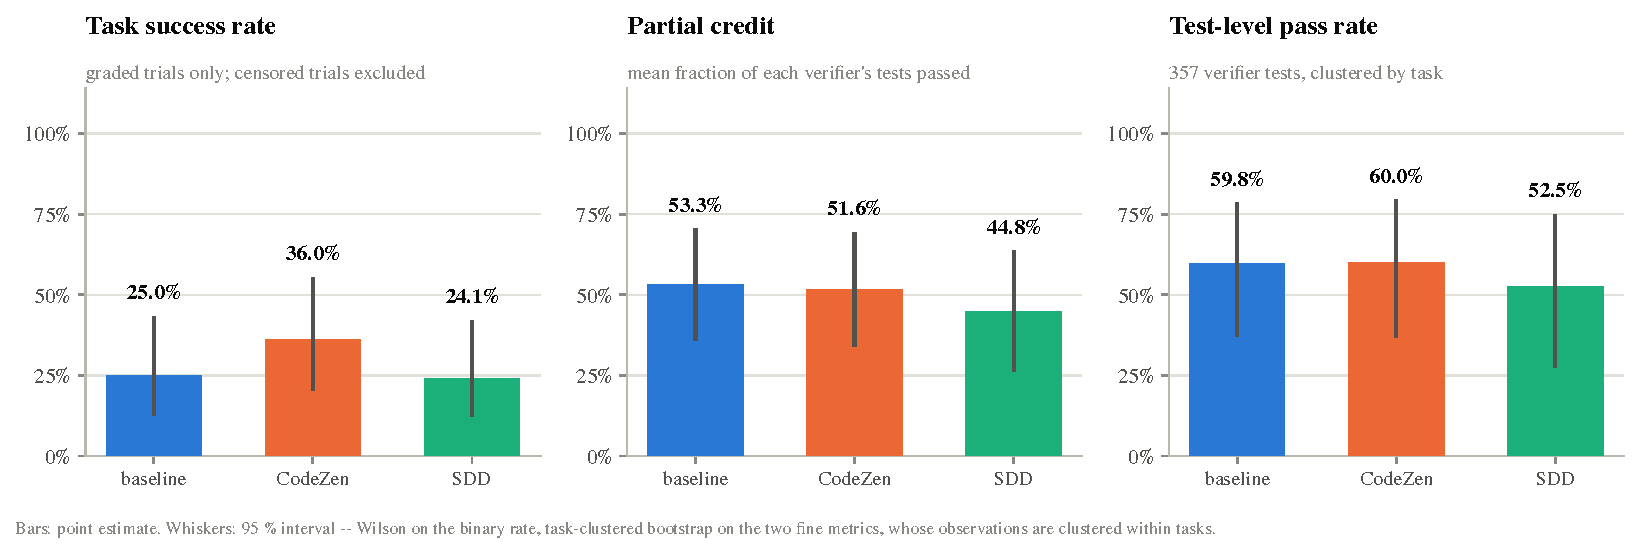
\includegraphics[width=\linewidth]{figures/suite-01-outcome.pdf}\\[0.4em]
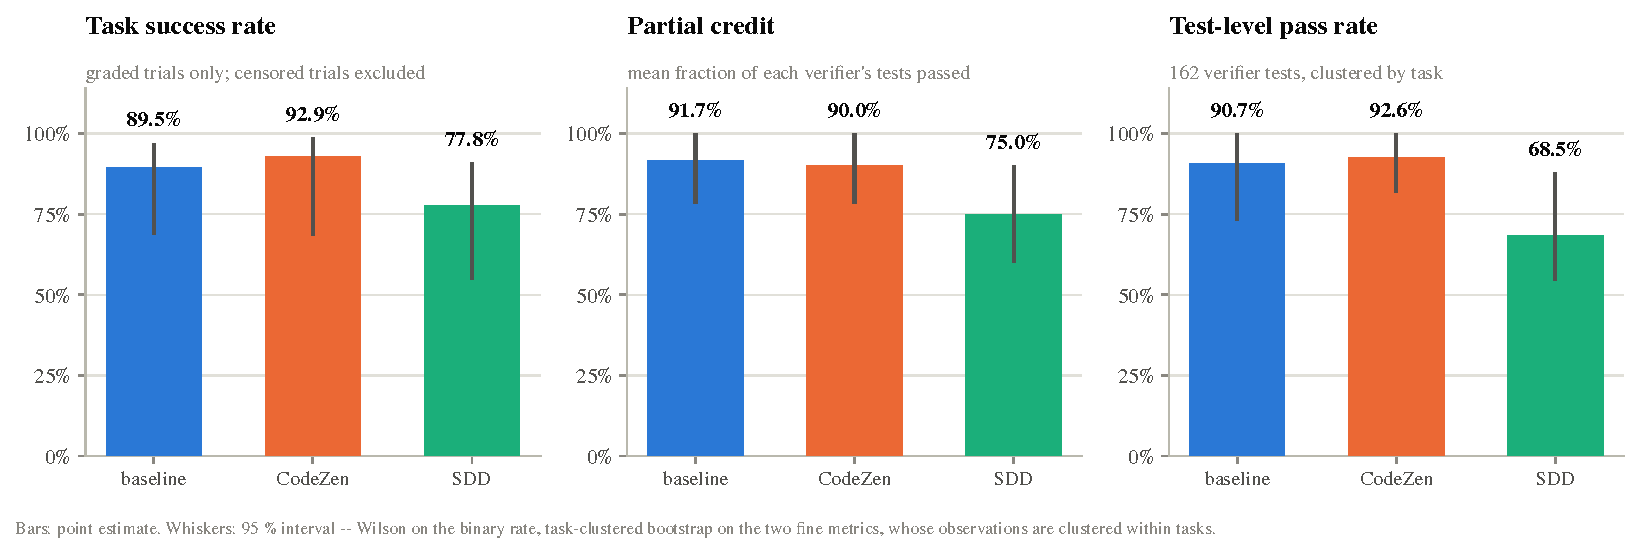
\includegraphics[width=\linewidth]{figures/ceiling-01-outcome.pdf}
\caption{Outcome by condition. Top: \emph{suite}. Bottom: \emph{ceiling}. Intervals contain
each other in every comparison. The one panel worth taking seriously is the bottom right: SDD
satisfies 22 points less of each \emph{ceiling} verifier than baseline does. Whiskers on the
test-level panels are task-clustered bootstrap intervals, not binomial intervals on test
rows.}
\label{fig:outcome}
\end{figure}

\textbf{On the \emph{suite} population the coarse and fine metrics disagree, and that is the
finding.} Success rate ranks CodeZen first by 11 points --- on a difference of two trials.
Partial credit, one continuous score per trial instead of one bit, ranks baseline first by
0.017 --- but exactly one trial in the 156 has no per-test record at all
(\task{torch-tensor-parallelism} under baseline, not censored, verifier ran 436.8\,s and
returned reward 0 with no test rows), so baseline's 0.533 is a mean over 31 trials. Scoring
that failure 0 gives 0.517 against CodeZen's 0.516, and the ordering becomes a tie; CodeZen's
paired ratio moves from $0.96\times$ to $1.00\times$. Test-level pass rate reproduces neither
ordering either: CodeZen is 0.2 points above baseline (60.0\,\% against 59.8\,\%), a coin
flip, and the only structure in that panel is SDD's 7-point shortfall. If a methodology effect existed and the binary reward were merely too
coarse to see it, partial credit is where it would appear first. What the fine metrics show is
not an absence --- the intervals are wide enough for a moderate real effect either way --- but
no detectable effect that the coarse and fine metrics agree about, and no fine-metric
ordering that survives one unrecorded trial except SDD's shortfall ($0.83\times$ and
$0.87\times$ under the two readings). Exact McNemar under pass-at-2 gives $p = 0.625$ for
CodeZen and $p = 1.000$ for SDD.

The 357 test rows are not 357 independent observations: they cluster inside 16 tasks, two of
which supply 30\,\% of them. Resampling whole tasks gives design effects of 5.7--7.4 and
effective sample sizes of 16--20, so the clustered intervals ([37.1, 78.6], [36.8, 79.5],
[27.3, 75.0]) are 42--48 points wide where binomial ones on the same counts are 17--18. Partial credit buys resolution;
the pooled test count does not buy power.

\textbf{The censoring convention compresses the \emph{suite} ordering rather than reversing
it.} Under reading 2 the rates are 21.9\,\%, 28.1\,\% and 21.9\,\%; under reading 3 they are
25.0\,\%, 34.4\,\% and 21.9\,\%. CodeZen's lead falls from 11 points to 6 and baseline ties
SDD. Three of the \emph{suite} kills --- \task{path-tracing} under baseline,
\task{adaptive-rejection-sampler} and \task{torch-tensor-parallelism} under CodeZen --- were
killed with a \emph{passing} verifier on disk, so readings 2 and 3 do not bracket an
uncertainty about them; they record three solved tasks as failures and as passes on identical
evidence. That is a harness defect, not a robustness check (\S\ref{sec:clock}).

\textbf{The ordering that is not in dispute is the price.} CodeZen spent \$68.13 against
\$21.87 and \$24.89 --- $3.11\times$ baseline, \$7.57 per graded pass against \$3.12 and
\$3.56 --- to buy a two-trial lead no test separates from noise, with partial credit and
test-level rate level with or below baseline's. As a hypothesis test this is a null; as a
procurement decision it is not neutral (\S\ref{sec:cost}).

\textbf{On the \emph{ceiling} population no ordering is a result} --- the population was
selected to be at ceiling and every McNemar $p$ is 1.000. What that run does establish about
outcome is that the censoring convention flips the ranking: CodeZen goes from 92.9\,\% (first)
under reading 1 to 80.0\,\% (second) under reading 3 and 65.0\,\% (\emph{third}) under
reading 2, a 27.9-point swing, because it was killed on 6 of 20 trials against baseline's 1.
Four of the nine kills in that run had already scored 1.0, three of them CodeZen's, so most of
that swing is the convention and not the methodology: no convention is right and a third
option is better than all of them (\S\ref{sec:clock}).

\textbf{The one fine-grained signal worth carrying forward is SDD's.} Partial credit 0.750
against baseline's 0.917, test-level pass rate 68.5\,\% against 90.7\,\% --- a 22-point gap
over 54 verifier tests per condition, and the same shortfall ($0.82$--$0.83\times$) appears
independently on both populations. Clustered by task the unpaired intervals still overlap
([54.4, 88.0] against [72.9, 100.0]), so the claim rests on the pairing, which never reaches
significance either ($p = 0.125$ at $n = 10$, lower on 4 of 10 tasks and higher on 1).
The consistency across two disjoint task sets is more interesting than either $p$-value, and
\S\ref{sec:adherence} supplies a mechanism.

\subsection{Why neither population could have shown an outcome effect}
\label{sec:screen}

Ten of the 16 \emph{suite} tasks are concordant under pass-at-2, seven of them failed by every
condition, and those ten consumed \textbf{\$74.47 of \$114.90}. Eight of the 10 \emph{ceiling}
tasks are concordant by construction. Effective $n$ per paired outcome test is 4--5 and 1--2.

This is not bad luck. Both populations came from a screen whose inclusion rule was applied on
\textbf{one} baseline trial per candidate, and one trial cannot distinguish \emph{always
fails} --- a floor task that carries no information --- from \emph{sometimes fails}, the only
kind of task that discriminates. Recent evidence makes that quantified rather than suspected:
across roughly 60{,}000 agent trajectories on SWE-Bench-Verified, single-run performance
estimates vary substantially between runs, including at temperature zero
\citep{bjarnason2026randomness}. A one-trial screen samples run-to-run noise as much as task
difficulty.

\begin{figure}[htbp]
\centering
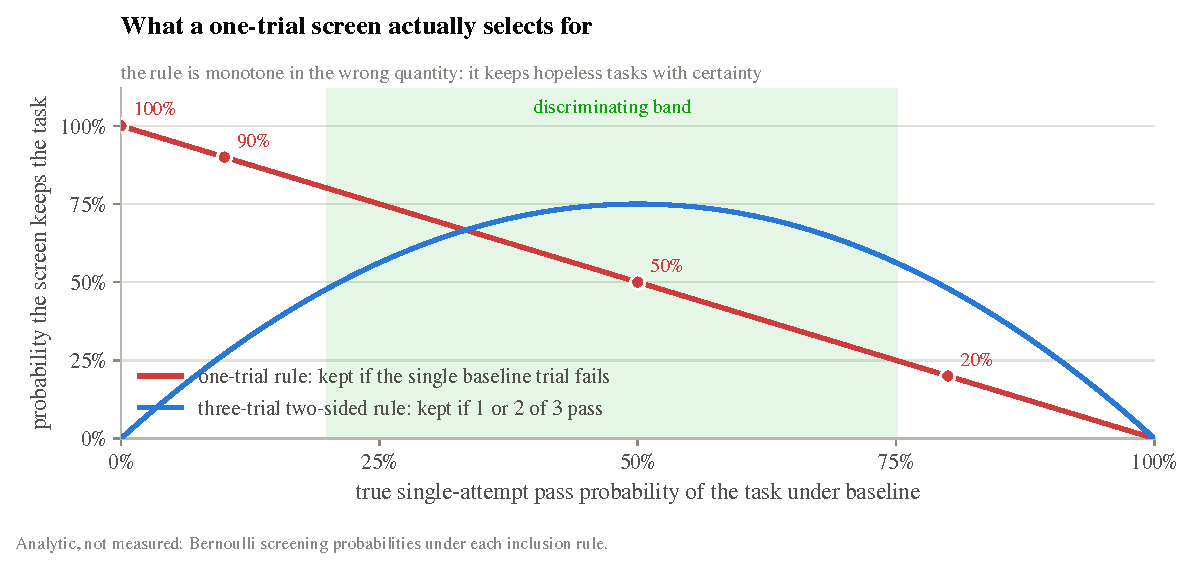
\includegraphics[width=0.82\linewidth]{figures/x13-screen-selection.pdf}
\caption{The defect, analytically. The red curve is the probability that a task with true
single-attempt pass probability $p$ survives the rule ``keep it if one baseline trial fails''.
It is monotone in the wrong quantity: it keeps hopeless tasks with certainty and discards half
of the ideally discriminating ones. The blue curve is a two-sided rule on three trials.}
\label{fig:screen}
\end{figure}

\begin{finding}{The most transferable lesson in the experiment is about experiments}
Three runs, three overshoots. Selecting tasks for human-expert difficulty produced a ceiling
(baseline 81\,\%). Screening for ``the bare agent fails'' produced a floor (37.5\,\%, seven
tasks failed by everything). The rejected set is a ceiling by construction (90\,\%). The fix
is a two-sided rule on the baseline pass \emph{rate} --- keep a task when 1 or 2 of 3 baseline
trials pass --- which costs three baseline trials per candidate instead of one.

Both runs also contain direct evidence that the one-trial rule misclassifies in \emph{both}
directions: \task{make-mips-interpreter} was excluded as ``the bare agent already passes it'',
and baseline then failed both of its attempts.

The uncomfortable possibility, stated plainly: the discriminating band may be narrow and
unstable, in which case no affordable screen produces a well-powered outcome comparison, and
cost and conformance should be promoted to primary endpoints with outcome demoted to
secondary. Both runs are consistent with that. Neither establishes it.
\end{finding}

\clearpage
\section{What process costs}
\label{sec:cost}

Cost is a continuous per-trial quantity rather than a rare binary event, so it is measurable
at $n = 10$--$16$ where the outcome is not. This is where the experiment delivers. Treating it
as a primary endpoint follows the shift described in \S\ref{sec:related}\,D: process machinery
is not automatically worth its price \citep{zhang2026tooltax,liu2026costbench}, and the
question is not whether it is expensive but what the price buys, on which tasks
\citep{snell2024scaling}.

\begin{figure}[htbp]
\centering
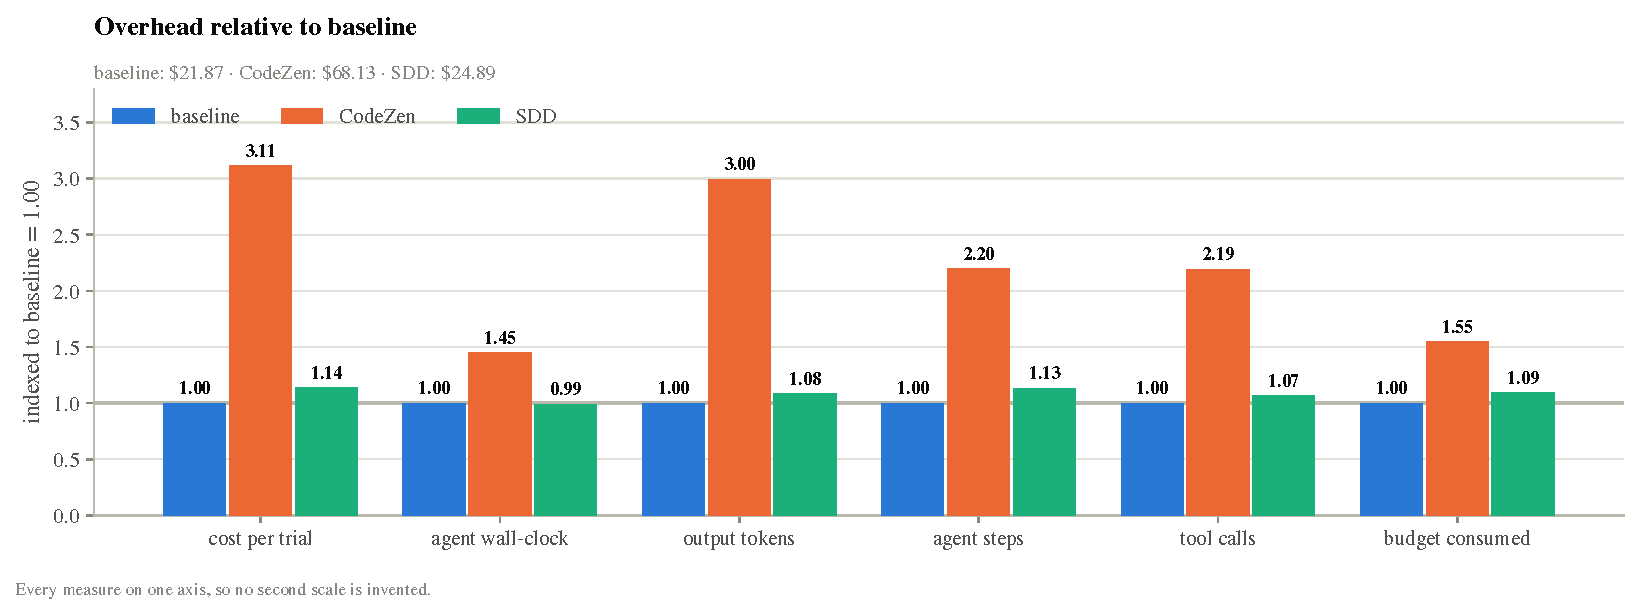
\includegraphics[width=\linewidth]{figures/suite-03-overhead.pdf}\\[0.4em]
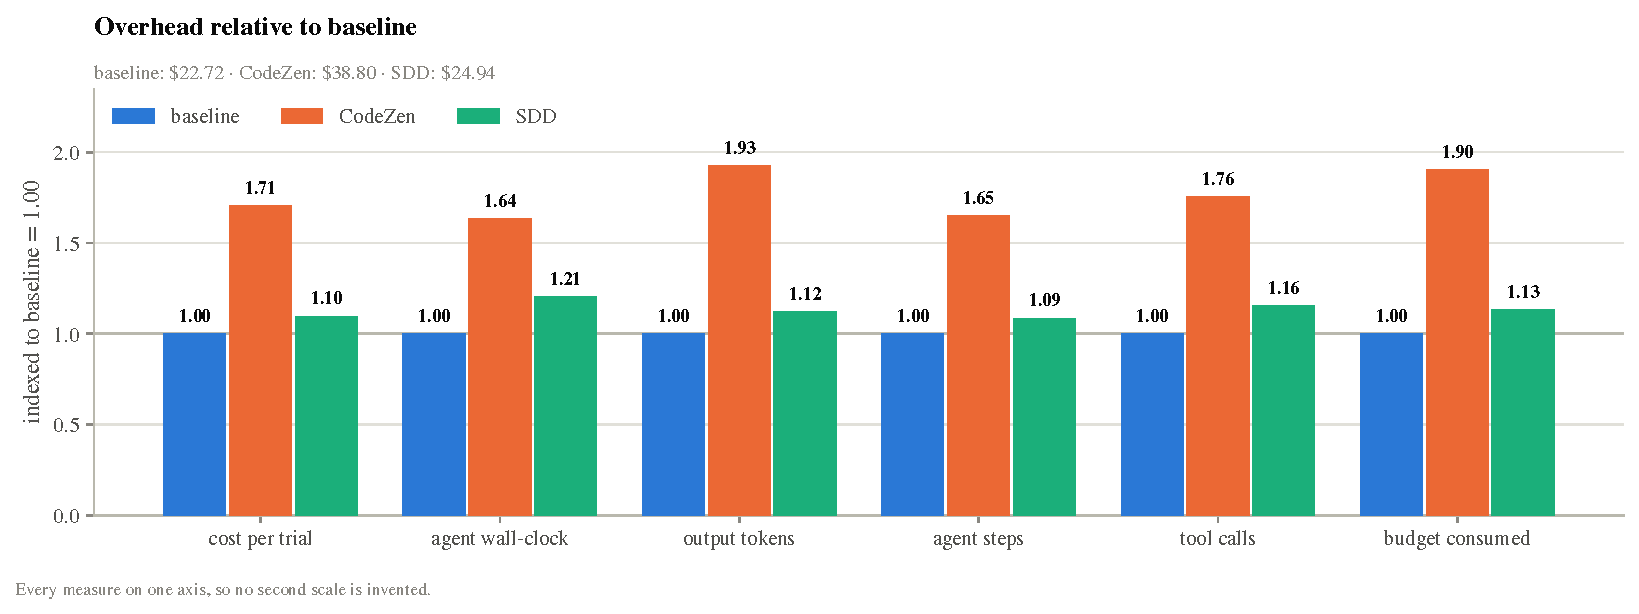
\includegraphics[width=\linewidth]{figures/ceiling-03-overhead.pdf}
\caption{Overhead indexed to baseline. Top: \emph{suite}, where work mostly aborts. Bottom:
\emph{ceiling}, where work mostly completes. Every measure sits on one axis, so no second
scale is invented. SDD is within noise of baseline on both populations; CodeZen is not.}
\label{fig:overhead}
\end{figure}

\begin{table}[htbp]
\centering
\caption{Paired tests. ``on'' counts the tasks where the condition exceeded baseline. Bold
marks $p < 0.05$. CodeZen is dearer on \emph{every} \emph{ceiling} task on cost, budget and
tokens; $p = 0.002$ is the minimum attainable value at $n = 10$.}
\label{tab:paired}
\scriptsize
\resizebox{\linewidth}{!}{
\begin{tabular}{@{}lrcrrcrrcrrcr@{}}
\toprule
 & \multicolumn{6}{c}{\textbf{suite} ($n = 16$ tasks)} & \multicolumn{6}{c}{\textbf{ceiling} ($n = 10$ tasks)} \\
\cmidrule(lr){2-7}\cmidrule(lr){8-13}
 & \multicolumn{3}{c}{CodeZen} & \multicolumn{3}{c}{SDD} & \multicolumn{3}{c}{CodeZen} & \multicolumn{3}{c}{SDD} \\
\cmidrule(lr){2-4}\cmidrule(lr){5-7}\cmidrule(lr){8-10}\cmidrule(lr){11-13}
vs baseline & ratio & on & $p$ & ratio & on & $p$ & ratio & on & $p$ & ratio & on & $p$ \\
\midrule
cost & 3.11$\times$ & 12/16 & \textbf{0.009} & 1.14$\times$ & 9/16 & 0.821 & 1.71$\times$ & 10/10 & \textbf{0.002} & 1.10$\times$ & 7/10 & 0.275 \\
budget consumed & 1.55$\times$ & 10/16 & 0.093 & 1.09$\times$ & 6/16 & 0.782 & 1.90$\times$ & 10/10 & \textbf{0.002} & 1.13$\times$ & 6/10 & 0.375 \\
output tokens & 3.00$\times$ & 12/16 & \textbf{0.015} & 1.08$\times$ & 10/16 & 0.668 & 1.93$\times$ & 10/10 & \textbf{0.002} & 1.12$\times$ & 6/10 & 0.375 \\
sub-agents spawned & 84.00$\times$ & 6/16 & \textbf{0.027} & 0.00$\times$ & 0/16 & 0.317 & 51.00$\times$ & 4/10 & 0.125 & 1.00$\times$ & 0/10 & 1.000 \\
partial credit & 0.96$\times$ & 6/16 & 1.000 & 0.83$\times$ & 4/16 & 0.440 & 0.98$\times$ & 1/10 & 0.750 & 0.82$\times$ & 1/10 & 0.125 \\
\bottomrule
\end{tabular}
}
\end{table}

\begin{finding}{The cost finding, as an operator needs it}
CodeZen costs \textbf{$1.71\times$} baseline on work it completes and \textbf{$3.11\times$} on
work it does not, for $0.96$--$1.00\times$ the partial credit --- level, once the one baseline
trial with no per-test record is counted as the failure it was. The second number is the one
that bites, because the methodology cannot tell in advance which kind of task it is on.
\end{finding}

\noindent The two multipliers are not in conflict --- they measure overhead on different
things. On the floor population CodeZen's trials frequently run to the wall without producing
a passing artefact, so the ratio includes work spent on tasks nothing solved. On the ceiling
population the same machinery runs on tasks that finish, and the overhead settles at
$1.71\times$.

\begin{figure}[htbp]
\centering
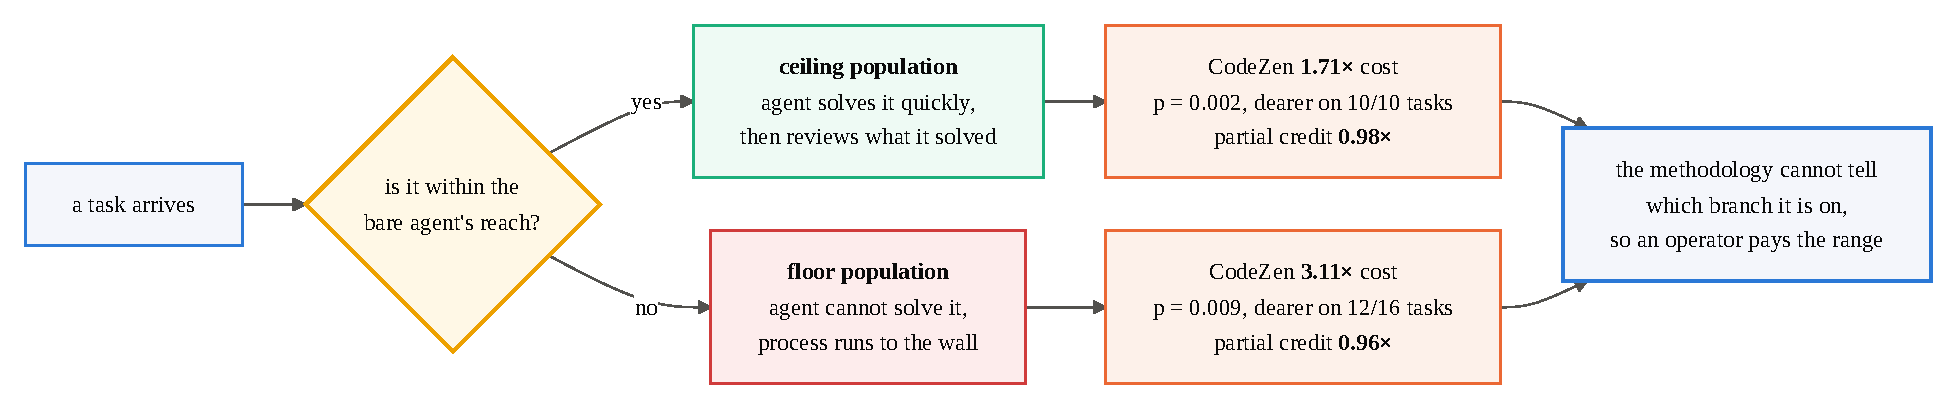
\includegraphics[width=\linewidth]{diagrams/d04-overhead-dynamics.pdf}
\caption{Why one toolkit yields two multipliers, and why an operator pays the range rather
than either endpoint.}
\label{fig:dynamics}
\end{figure}

Three supporting facts close off the obvious objections.

\textbf{The smaller run is the stronger evidence.} Ten of ten tasks dearer on four separate
metrics beats twelve of sixteen, because there is no task where the effect is absent and no
runaway trial can be carrying the mean. Per-task cost ratios range from $1.01\times$ to
$10.6\times$ in \emph{ceiling} and $0.06\times$ to $16.0\times$ in \emph{suite}.

\textbf{It is not a caching artefact.} Cache hit ratios are effectively identical across
conditions (94.8/94.5/93.4\,\% in \emph{suite}; 96.0/95.8/96.1\,\% in \emph{ceiling}) and
thinking share of output is flat. The extra spend is extra work.

\textbf{SDD's cost is not the story; its partial credit is.} $1.10$--$1.14\times$ spend is
indistinguishable from baseline in both runs ($p = 0.82$, $p = 0.28$). The shortfall is in
what it satisfied, not what it spent (\S\ref{sec:outcome}, \S\ref{sec:adherence}).

\subsection{The multiplier is flat in task length; the bill is not}

\begin{figure}[htbp]
\centering
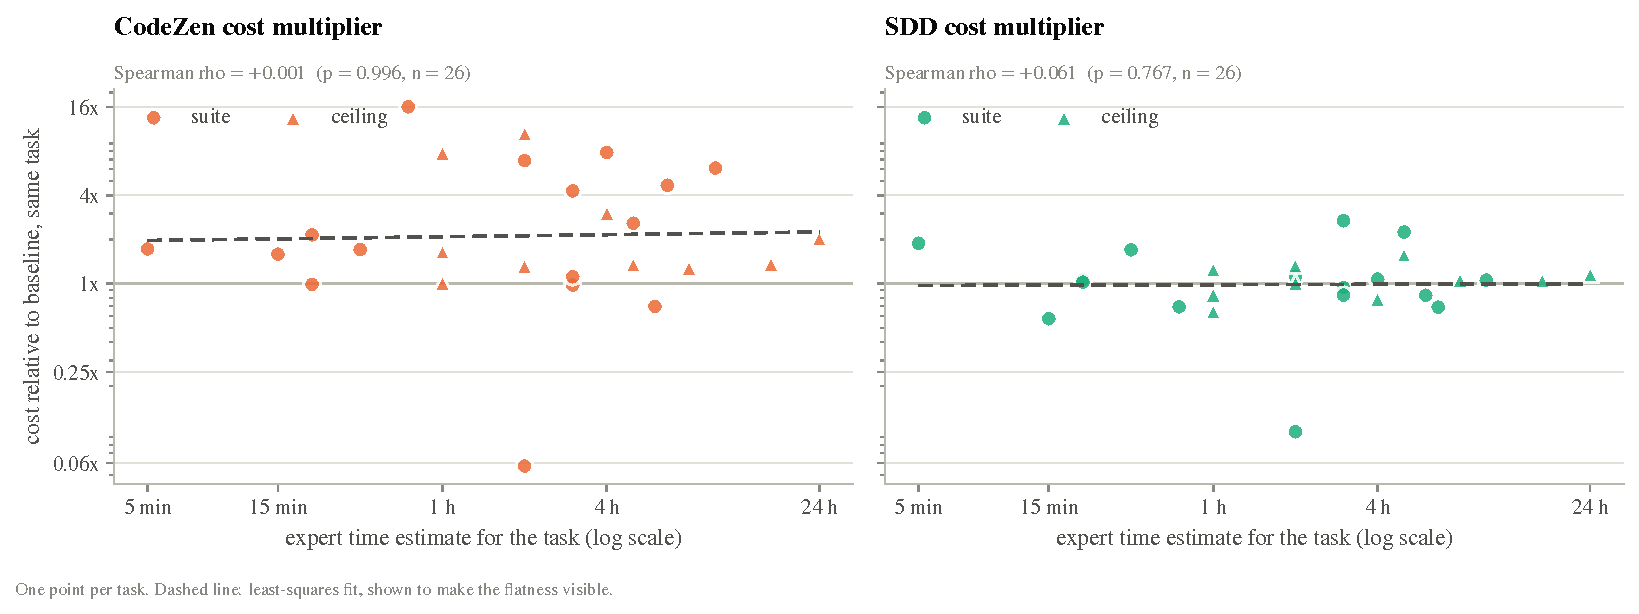
\includegraphics[width=\linewidth]{figures/x07-cost-ratio-vs-length.pdf}
\caption{The cost \emph{multiplier} against expert time estimate, pooled over both runs and a
$288\times$ range of task length. A Spearman $\rho$ of $+0.001$ against that range is as close
to a flat line as this data can produce: process overhead is proportional, not
super-proportional.}
\label{fig:flat}
\end{figure}

The absolute penalty grows only because the base grows: baseline cost against
$\log_{10}$(expert minutes) gives $\rho = +0.696$, $p < 0.001$, the strongest correlation in
the pooled data. CodeZen's mean overhead is \textbf{\$0.79 per trial on short-budget tasks and
\$1.68 on long-budget ones} --- twice the dollars for the same multiplier. So the intuition
that long tasks are less feasible under a methodology is right, but not for the reason usually
given: a constant multiplier on a larger base is simply a larger bill. The sharper half of the
feasibility problem is not the bill at all.

\clearpage
\section{The clock is the binding constraint}
\label{sec:clock}

Human engineering already treats review latency as a first-class cost
\citep{kudrjavets2024review}. An agent sharpens the trade-off, because review and
implementation draw on the \emph{same} bounded budget rather than on different people's
calendars --- and that budget is denominated in the units used to define agent time horizons
\citep{kwa2025horizons}. Whether exhausting it actually dominated here is this section's
result, not a prior.

\begin{center}\small
\begin{tabular}{@{}llrrrr@{}}
\toprule
Run & Condition & Mean budget & Median & Trials over 75\,\% & Killed by the clock \\
\midrule
\multirow{3}{*}{\emph{suite}}
 & \code{baseline} & 30.2\,\% & 15.4\,\% & 5 & 4 of 32 \\
 & \code{codezen-viable} & \textbf{46.8\,\%} & 36.7\,\% & \textbf{9} & \textbf{7 of 32} \\
 & \code{sdd} & 33.1\,\% & 15.8\,\% & 6 & 3 of 32 \\
\midrule
\multirow{3}{*}{\emph{ceiling}}
 & \code{baseline} & 30.2\,\% & 27.5\,\% & 1 & 1 of 20 \\
 & \code{codezen-viable} & \textbf{57.5\,\%} & 56.2\,\% & \textbf{7} & \textbf{6 of 20} \\
 & \code{sdd} & 34.3\,\% & 22.8\,\% & 3 & 2 of 20 \\
\bottomrule
\end{tabular}
\end{center}

\begin{figure}[htbp]
\centering
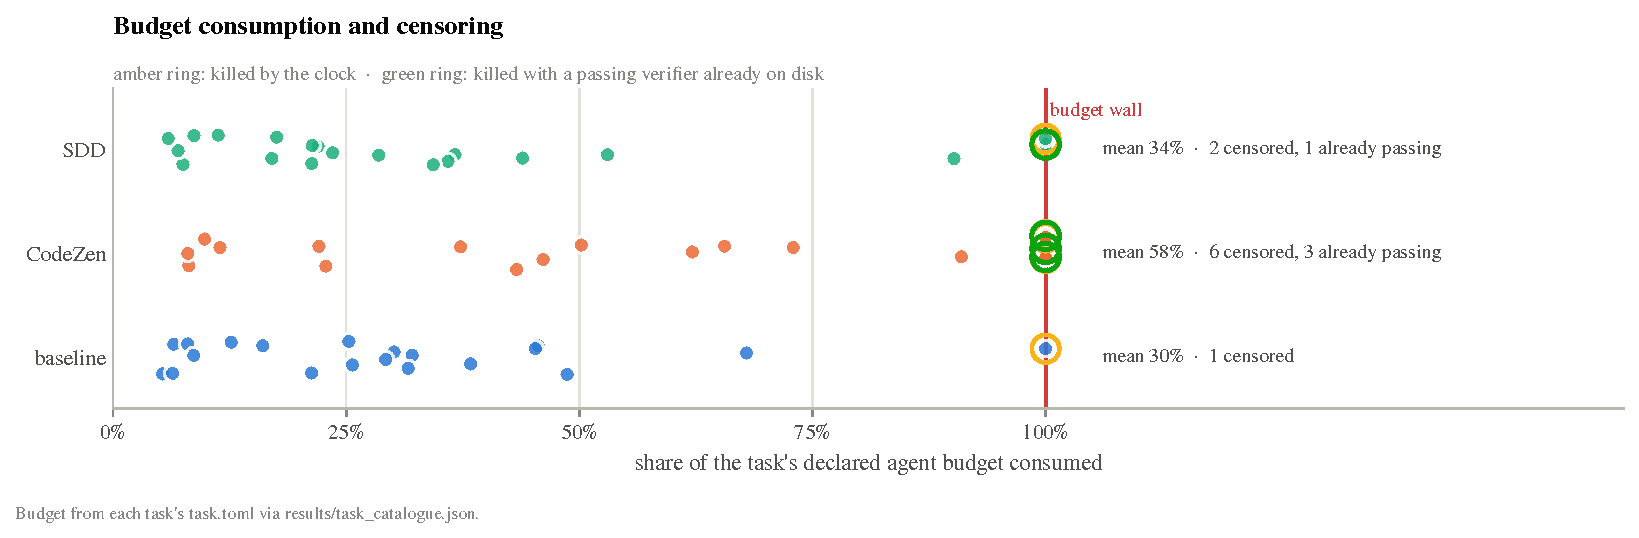
\includegraphics[width=\linewidth]{figures/ceiling-04-budget.pdf}
\caption{\emph{ceiling}: budget consumption and censoring. Each dot is a trial, positioned by
the share of its task's declared budget it consumed. Amber rings were killed by the clock;
green rings were killed with a passing verifier already on disk. This is the population where
the whole causal chain is visible, because the work mostly completes.}
\label{fig:budget}
\end{figure}

\begin{finding}{The chain, measured rather than inferred}
\begin{enumerate}[nosep]
\item CodeZen delegates --- 2.55 sub-agents per trial against baseline's 0.05 --- and reviews
      after implementing.
\item That work is real and takes wall-clock, so budget consumption rises $1.90\times$
      ($p = 0.002$, higher on 10 of 10 tasks).
\item On tasks whose budget is tight relative to their size, the extra consumption crosses the
      wall and Harbor kills the agent: \textbf{25\,\% of CodeZen's 52 trials} against 9.6\,\%
      for baseline and SDD.
\item Sometimes the work was already done. Sometimes it was not.
\end{enumerate}
\end{finding}

\subsection{Censoring is throwing away observations that already exist}

\begin{figure}[htbp]
\centering
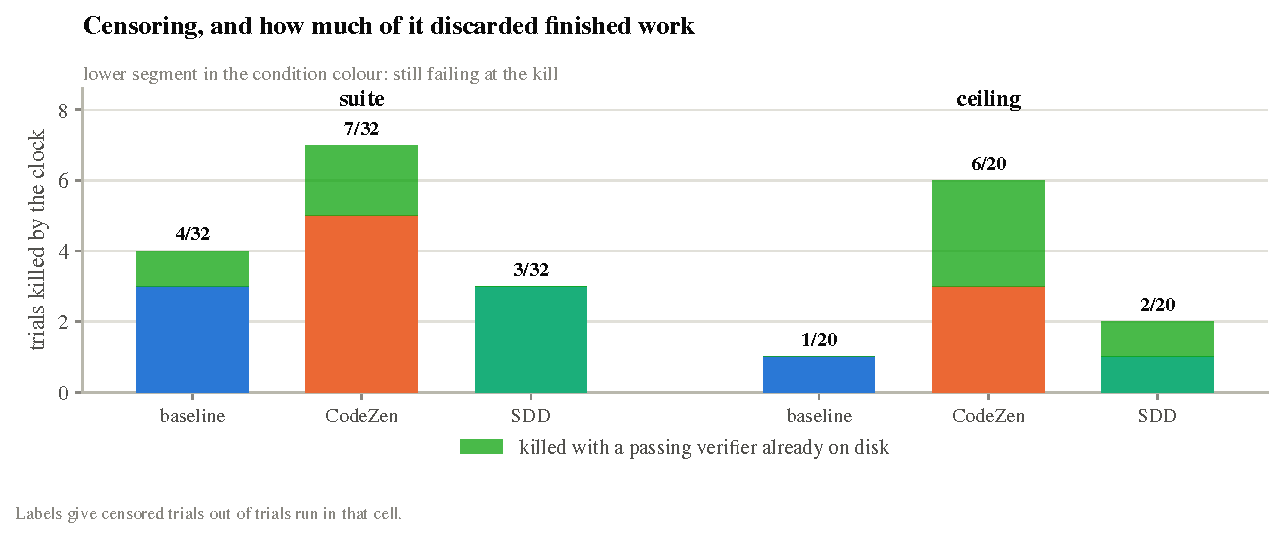
\includegraphics[width=0.9\linewidth]{figures/x08-censoring.pdf}
\caption{Every trial killed by the clock, split by what the verifier scored on the workspace
that was killed. Seven of 23 --- 30.4\,\% --- discarded a solution that had already passed
every test.}
\label{fig:censoring}
\end{figure}

A Harbor timeout is right-censoring: the trial stopped before the event of interest, so the
observation is a bound rather than a result, and censored observations carry information that
ordinary statistics discard \citep{leung1997censoring}. The analogy stops there --- the
censoring mechanism is \emph{informative}, since the agent's own behaviour determines whether
it reaches the deadline --- so this is a reason to record the disk state at the kill, not a
licence to apply survival analysis off the shelf.

Across both runs 23 trials were killed and \textbf{7 scored reward 1.0}. Under the censoring
convention all 23 vanish from the analysis; under ``timeout = failure'' all 23 count against
their condition; under kill-time grading, seven of them are successes. Harbor already recorded
those seven verdicts, so kill-time grading costs no model tokens, turns a lost observation
into a measured one, and removes the need to choose between dropping a trial and overruling
its verifier. Adopting it as the primary endpoint is the single cheapest improvement available
to this design.

\subsection{The post-completion trap}
\label{sec:trap}

\begin{figure}[htbp]
\centering
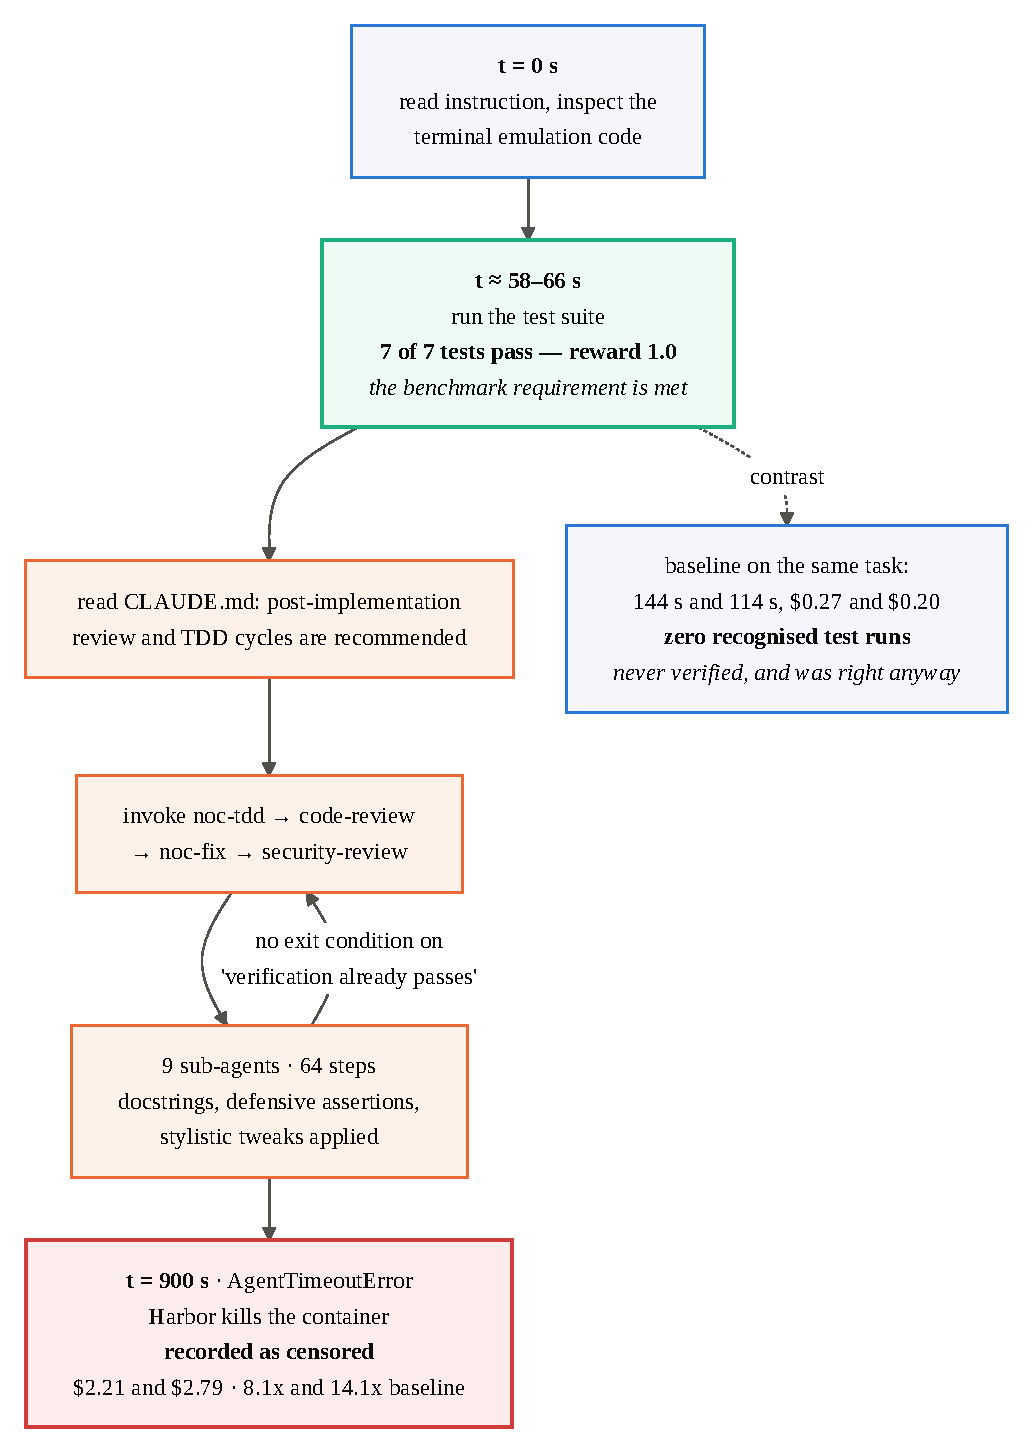
\includegraphics[width=0.78\linewidth]{diagrams/d03-post-completion-trap.pdf}
\caption{\task{headless-terminal} under CodeZen, minute by minute. The benchmark requirement
was met at 65.6\,s on one attempt and 58.5\,s on the other. The remaining 834 seconds were
ceremonial, until Harbor's wall-clock killed the container and both trials were recorded as
censored --- despite scoring reward 1.0.}
\label{fig:trap}
\end{figure}

\noindent The single most illuminating trajectory in the dataset is \task{headless-terminal}
under CodeZen (Figure~\ref{fig:trap}), and it is not a story about difficulty. The contrast
with baseline is sharper than ``one condition was thorough and one was not''. Baseline finished the same task in \textbf{144.5\,s and 114.1\,s for \$0.27 and
\$0.20}, and ran \textbf{zero recognised test invocations} on either attempt: it edited the
code, stopped, and was right anyway. CodeZen did the responsible thing --- it ran the tests,
and they passed inside 66 seconds --- and then spent another 834 seconds and \$2.21/\$2.79
(that is $8.1\times$ and $14.1\times$ baseline) applying docstrings, defensive assertions and
stylistic tweaks across nine sub-agents. On this task the entire cost difference bought the
agent a confirmation it then failed to act on.

\begin{finding}{The architectural lesson}
An autonomous agent under a real time or compute budget needs an \textbf{explicit exit
condition}. When verification already succeeds, procedural review skills must be suppressed,
or gated behind a strict time-remaining threshold. In human engineering, thoroughness and peer
review are virtues; in an agent with a fixed clock and no termination gate, thoroughness is a
failure mode.

Process research has long held that a standardised process should be tuned to its project
rather than applied unchanged \citep{xu2007tailoring}. An agent needs a strictly more dynamic
form of that: the context that gates the process is not only the project but the
\emph{execution state} --- whether the artefact already passes --- and the budget remaining.
\end{finding}

\noindent The same machinery, on tasks where the work was \emph{not} already done, is what
produces the $3.11\times$ multiplier. Baseline meets a hard barrier --- a missing shared
library, a numerical convergence problem, an obscure binary format --- tries a few commands
and stops inside about 20 steps and \$0.68. CodeZen treats failure as a signal to invoke
process: \code{noc-tdd} to write tests, \code{code-review} to inspect the non-working code,
\code{noc-fix} to attempt repairs. Because every sub-agent runs the \emph{same} model, they
share the parent's blind spots and cannot conjure domain knowledge the base model lacks; they
return detailed critiques and superficial syntactic suggestions, and the parent burns steps
until the clock expires. On \task{filter-js-from-html} that loop reached 100\,\% of budget on
both attempts at a $16.0\times$ cost ratio, with zero passing tests.

\subsection{One clean regression, stated honestly}

\begin{finding}{\task{torch-pipeline-parallelism}}
Baseline passes it on \textbf{one of two} attempts, using 29\,\% of its declared budget with 3
of 3 tests; its other attempt failed at 2 of 3 inside 38\,\%. CodeZen invoked
\code{code-review} on one attempt and \code{noc-tdd}\,+\,\code{code-review} on the other,
consumed \textbf{100\,\% of budget on both}, and failed both at 2 of 3. The task needs delicate
synchronisation across pipeline stages; the review sub-agents analysed code style and test
architecture while the synchronisation bug went unfixed.

The honest version of the claim is therefore ``a task baseline solves half the time, that
CodeZen never solved, at three times the budget'' --- not ``a task baseline solves easily''.
Under the reliability reading (pass-both) the regression list grows: CodeZen also loses
\task{schemelike-metacircular-eval}, and SDD loses three tasks it passed once and failed once.
\end{finding}

\clearpage
\section{Availability is not adherence}
\label{sec:adherence}

\begin{finding}{Whatever these runs measured, it was not a methodology being followed}
Every toolkit skill registered in every one of the 104 toolkit trials, and preflight proved
every instruction file present. A toolkit skill was invoked in 30 of them. \textbf{74 of 104
(71\,\%) invoked nothing.} CodeZen invoked one in 38\,\% of \emph{suite} and 35\,\% of
\emph{ceiling} trials; SDD in 22\,\% and 20\,\%.
\end{finding}

\begin{table}[htbp]
\centering
\caption{The five behavioural measures that carry a mechanism. Shell commands are bucketed by
pattern rather than parsed, so ``verification commands'' is a comparison between conditions on
one corpus, not an absolute count.}
\label{tab:behaviour}
\small

\begin{tabular}{@{}lrrrrrr@{}}
\toprule
 & \multicolumn{3}{c}{\textbf{suite}} & \multicolumn{3}{c}{\textbf{ceiling}} \\
\cmidrule(lr){2-4}\cmidrule(lr){5-7}
per-trial mean & baseline & CodeZen & SDD & baseline & CodeZen & SDD \\
\midrule
sub-agents spawned & 0.03 & 2.62 & 0.00 & 0.05 & 2.55 & 0.05 \\
verification commands & 0.56 & 3.56 & 0.66 & 0.30 & 1.65 & 0.00 \\
wrote its own test file & 9\% & 34\% & 3\% & 10\% & 25\% & 0\% \\
agent steps & 21.9 & 48.0 & 24.8 & 26.0 & 42.9 & 28.2 \\
tool results with an error & 10.2\% & 12.9\% & 9.7\% & 13.1\% & 16.9\% & 10.9\% \\
\bottomrule
\end{tabular}

\end{table}

\textbf{CodeZen's delegation is its entire cost signature.} 84 sub-agent spawns across its 32
\emph{suite} trials against 1 for baseline and 0 for SDD; 51 across its 20 \emph{ceiling}
trials. Each sub-agent inherits prompt context and produces its own thinking and output
tokens, which accounts for most of the step and token overhead in \S\ref{sec:cost}. It is also
invisible to the cell-level report, which has no delegation column --- and the
counter-position is worth noting: a deliberately simple localise--repair--validate pipeline
has been shown competitive with elaborate agent scaffolding on repository-level tasks
\citep{xia2024agentless}.

\textbf{CodeZen verifies far more, and it does not help.} The expectation under test is
well-supported --- TDD is associated with quality gains, at mixed-to-negative productivity
cost \citep{bissi2016tdd,tosun2017industry} --- so what follows is not evidence that testing
is harmful, but a question about whether that trade survives translation into an agent with a
fixed budget and no access to the grading oracle. 3.56 verification commands per trial against
baseline's 0.56 in \emph{suite} --- a $6.3\times$ increase, $p = 0.046$ --- and it wrote a
dedicated test file in 34.4\,\% of trials against baseline's 9.4\,\%. Partial credit still came
out $0.96\times$ baseline.

\begin{finding}{A hypothesis for why more testing did not mean more correctness}
\emph{Proposed, not measured.} The data establishes the disconnect between verification
activity and verified outcome; this is our account of it.

In an autonomous benchmark the verifier is an external oracle the agent cannot see. When an
agent writes its own tests it tests against its \emph{own} reading of the problem: if it has
misread an edge case, it encodes the misreading in a test, runs it, sees green, and believes
the solution is correct. The external verifier then tests the actual edge case and fails it.
On this reading, ungrounded test-driven development produces \textbf{false confidence}, and
testing is only as good as the specification it validates against. It is plausible rather than
merely available because agents are a distinct class of end user with their own failure modes
\citep{yang2024sweagent}. The instrument that would settle it is in \S\ref{sec:changes}: log a
``mock misalignment'' event whenever the agent's own suite passes and the verifier does not.
\end{finding}

\textbf{SDD points the wrong way on the one behaviour that matters.} It is near-invisible
otherwise --- steps $1.13\times$, tool calls $1.07\times$, wall-clock $0.99\times$, zero
sub-agents --- but on the \emph{ceiling} population it ran \textbf{zero} recognised
verification commands across 20 trials, against baseline's 0.30 and CodeZen's 1.65. For a
toolkit that ships an \code{sdd-verify} skill, and invoked it in two of its four skill-using
trials in that run, this is a direct counter-signal, and it lines up with the partial-credit
shortfall: SDD satisfied 68.5\,\% of verifier tests against baseline's 90.7\,\% and checked
its work less than the bare agent did. The caveat matters more here than anywhere else:
verification inside a heredoc is invisible to the pattern bucket, so 0.00 means ``no
recognised test invocation''. But the same bucket credits baseline with 0.30 and CodeZen with
1.65 on the same corpus, so the comparison stands even if the absolute count understates.

\subsection{Two invocation patterns, and one question this design cannot answer}

\textbf{CodeZen implements first and reviews after.} Ten of 12 \emph{suite} skill-using trials
and 5 of 7 \emph{ceiling} ones open with \code{noc-tdd}; \code{code-review} and
\code{security-review} appear \emph{after} the work rather than as a method for doing it. The
ordering matters, because the human TDD literature has itself struggled to separate the
benefit of testing \emph{first} from that of short verified cycles
\citep{fucci2017dissection}: a toolkit that invokes a test-first skill and then implements in
one pass is not obviously practising the thing the evidence supports.

\textbf{SDD's chain either runs completely or aborts at step two.} Five trials across both
runs stop after \code{sdd-specify} and \code{sdd-clarify} having consumed 2.2--17.0\,\% of
budget, and a sixth stops after \code{sdd-specify} alone at 23.4\,\%. The agent opened the
process, produced a specification, and did not follow it --- reverting to unassisted coding
with cluttered context and lost time.

\begin{finding}{Does invoking the methodology predict failure? Selection and effect cannot be separated}
Pooled over both runs, 30.0\,\% of skill-invoking trials passed against 54.1\,\% of toolkit
trials that invoked nothing. Two explanations both have support and this design cannot
distinguish them:

\emph{Distress} --- when the agent grasps a solution it edits files and runs commands, ignoring
the skills directory; when it is stuck it reaches for documented process as a fallback, so the
low pass rate is a property of the tasks those trials were on. \S\ref{sec:length} adds direct
evidence for this: SDD's invocation rate rises with task size.

\emph{Consumption} --- invoking the chain spends the budget that would have solved the task.
The censoring data supports this independently.

Only a design that \textbf{randomises invocation} separates them, and no run in this sequence
has done that. It is also what ``methodology \emph{enforcement}'' literally requires.
\end{finding}

\clearpage
\section{The length hypothesis, and the paradox inside it}
\label{sec:length}

Human expert completion time is the axis on which agent evaluation defines a task-completion
horizon --- the duration at which an agent is predicted to succeed with a given reliability
\citep{kwa2025horizons} --- so it is both the natural predictor here and the one the benchmark
supplies. The hypothesis that motivated pooling the two runs was that structure should become
more valuable as tasks grow longer. It is testable on the pooled 26 tasks, whose expert estimates
span 5 to 1{,}440 minutes, 10 of them carrying Terminal-Bench's own \code{long-horizon} axis.

\begin{table}[htbp]
\centering
\caption{The six pooled correlations the section argues from. At $n = 26$, 80\,\% power needs
$|\rho| \ge 0.53$, so every row below that means ``not resolved'', not ``absent''.}
\label{tab:corr}
\small

\begin{tabular}{@{}lrrl@{}}
\toprule
Spearman, pooled over 26 tasks & \multicolumn{1}{c}{$\rho$} & \multicolumn{1}{c}{$p$} & what it says \\
\midrule
baseline pass-at-2 vs log expert time & $-0.078$ & 0.704 & human difficulty does not predict agent difficulty \\
baseline absolute cost vs log expert time & $+0.696$ & \textbf{$<$0.001} & longer tasks cost more, as expected \\
CodeZen cost \emph{ratio} vs log expert time & $+0.001$ & 0.996 & the multiplier is flat over $288\times$ of length \\
$\Delta$ pass-at-2, CodeZen, vs expert/budget & $+0.330$ & 0.099 & the only lean in the hypothesis' direction \\
$\Delta$ partial credit, CodeZen, vs expert/budget & $-0.020$ & 0.923 & \dots and it is gone at 519 graded tests \\
SDD toolkit skill calls vs log expert time & $+0.379$ & 0.056 & SDD gates itself on perceived task size \\
\bottomrule
\end{tabular}

\end{table}

\begin{figure}[htbp]
\centering
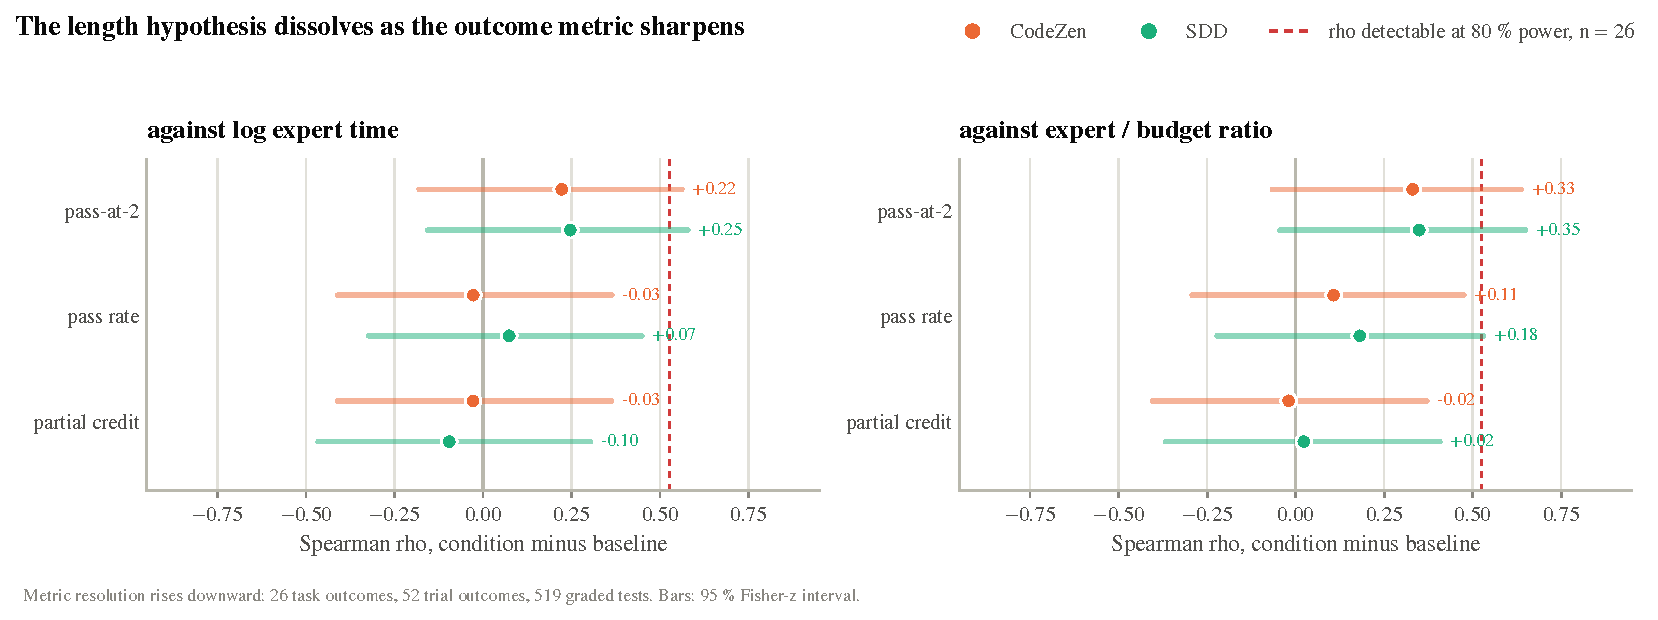
\includegraphics[width=\linewidth]{figures/x10-length-dissolution.pdf}
\caption{The length effect as a function of metric resolution. Reading downward, the outcome
measure sharpens from 26 binary task outcomes to 52 binary trial outcomes to 519 graded
verifier tests. A real effect should sharpen with the instrument. This one dissolves --- and
for CodeZen against expert time it turns faintly negative.}
\label{fig:dissolution}
\end{figure}

There is a weak positive lean in the predicted direction and \emph{only in the coarsest
metric}: $\Delta$ pass-at-2 against the expert/budget ratio gives $\rho = +0.330$ (CodeZen)
and $+0.349$ (SDD), both just outside significance at roughly 35--40\,\% power. On pass
\emph{rate} it drops to $+0.107$ and $+0.181$. On partial credit it is indistinguishable from
zero. \textbf{That is the signature of noise in a coarse metric.} The data does not support the
hypothesis and is not powered to reject it.

Terminal-Bench's own axis says the same and adds something: on every finer-grained outcome
measure both toolkits do \emph{worse} on long-horizon tasks than on short ones. SDD's
partial-credit deficit is $-0.182$ on long-horizon tasks against $-0.080$ on short ones ---
its worst performance is exactly where its own documentation claims it should be strongest.

\begin{figure}[htbp]
\centering
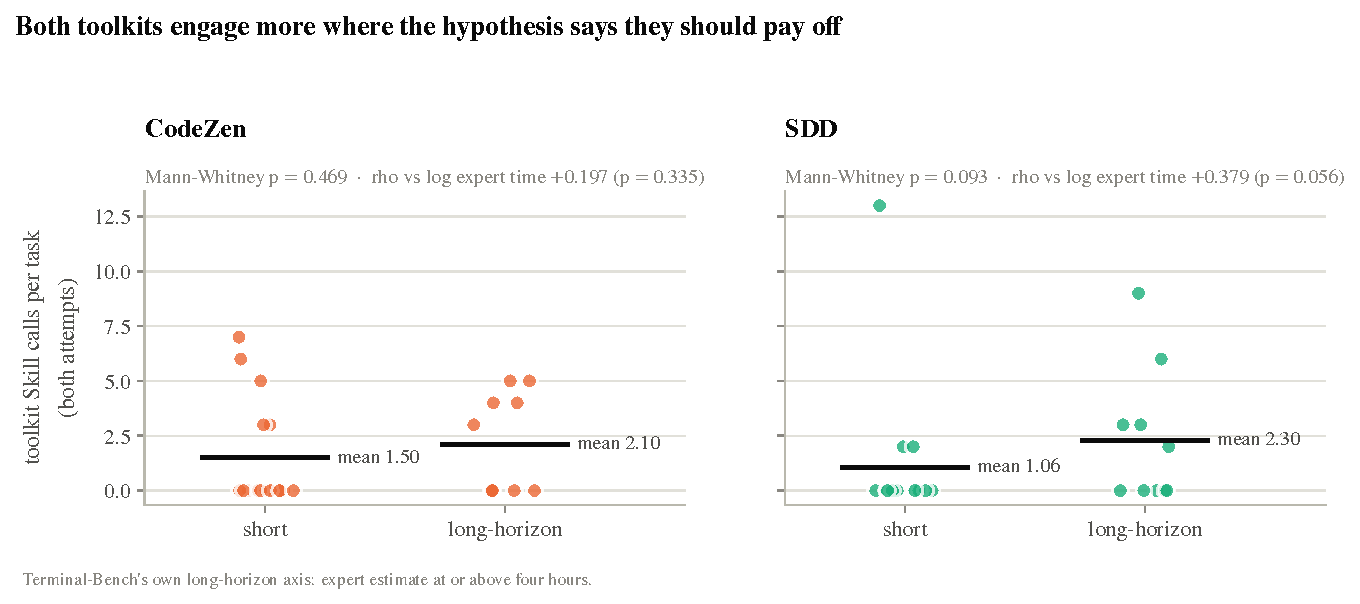
\includegraphics[width=0.9\linewidth]{figures/x11-adherence-vs-length.pdf}
\caption{Toolkit invocation against task horizon. SDD invokes its chain $2.2\times$ more often
on long-horizon tasks than on short ones ($\rho = +0.379$ against log expert time,
$p = 0.056$). It gates itself on perceived task size, and engages exactly where the hypothesis
says it should pay off.}
\label{fig:selfgate}
\end{figure}

\begin{finding}{The most pointed result in the dataset}
This is not ``we could not find the effect where we looked''. It is ``the toolkit looked in
the same place, acted on the same belief, and the belief did not pay''. SDD gates itself on
task size, engages its process where the length hypothesis predicts a payoff, spends budget
and context authoring specifications, decouples from empirical verification --- and posts the
largest partial-credit deficit anywhere in the data on precisely those tasks.

It also settles an older question. A harness that gave the agent no reason to consult a process
would suppress invocation \emph{uniformly}. Invocation instead rises with perceived task size,
so the low adherence of \S\ref{sec:adherence} is at least partly the toolkit gating itself.
\end{finding}

\noindent \textbf{Two limits on this analysis.} The pooled sample mixes two populations
selected on baseline outcome, so run membership dominates baseline pass rate more than
long-horizon status does; long-horizon tasks split 5/5 between the runs, so the confound is not
aligned with the predictor but is not orthogonal either. And the length range is not the range
the hypothesis is about: these tasks top out at a day of expert time in a \emph{single
autonomous session with a fully specified instruction}, while the hypothesis concerns
multi-session work with ambiguous requirements and a human in the loop.

\clearpage
\section{``Just retry more'': plausible, not proven}
\label{sec:bestofn}

Repeated sampling is an established way to raise the functional correctness of model-written
code \citep{chen2021codex} and the accuracy of model reasoning
\citep{wang2023selfconsistency}, and dividing a fixed inference-time budget between one careful
attempt and several cheap ones is a research question in its own right
\citep{snell2024scaling}. The claim below is the software-process form of it.

The sharpest operational claim to come out of the independent review is that a fixed budget is
better spent on more independent attempts with the bare agent than on a methodology. The
argument is arithmetic: if a methodology trial costs $k$ baseline trials and baseline's
per-attempt pass rate is $p$, then at equal spend

\[ P(\text{at least one of } k \text{ passes}) = 1 - (1-p)^k, \]

which on the \emph{suite} population gives 59\,\% against CodeZen's 36\,\% for the same money.
The conclusion drawn was that repeated sampling \emph{strictly dominates} process.

\subsection{The assumption, and why it fails here}

That formula assumes every attempt on every task is an exchangeable draw from one common
Bernoulli rate --- which does not follow from the sampling results above, since those
establish that \emph{more samples help}, not that attempts on a fixed task are exchangeable.
Independent evidence says they are not \citep{bjarnason2026randomness}. The two-attempt design
tests the joint consequence directly, and it leans the wrong way in five of six
run $\times$ condition cells: observed pass-at-2 falls \emph{below}
the independence prediction (\emph{suite} baseline 0.375 against 0.438; SDD 0.313 against
0.390; CodeZen 0.500 against 0.569). No single cell rejects homogeneity at $n = 10$--$16$
tasks ($\chi^2$ on the 0/1/2 count distributions gives $p = 0.16$ to $0.57$), but the sign is
consistent and the mechanism is not in doubt: ten of sixteen \emph{suite} tasks were failed by
baseline on both attempts, and retries cannot rescue a task that is dead.

\subsection{Three estimators, and the range they produce}

\begin{table}[htbp]
\centering
\caption{Best-of-$N$ at equal spend. The condition keeps its actual two attempts; baseline
receives $2k$ attempts for the same money. \emph{Homogeneous} denies task heterogeneity (the
optimistic bound); \emph{plug-in} takes two-attempt per-task estimates at face value (the
pessimistic bound); \emph{beta-binomial} fits the heterogeneity by maximum likelihood.}
\label{tab:bestofn}
\small

\begin{tabular}{@{}lrrrrrr@{}}
\toprule
 & \multicolumn{1}{c}{baseline $\bar p$} & \multicolumn{1}{c}{$k$ at equal} &
 \multicolumn{3}{c}{baseline best-of-$k$, by estimator} & \multicolumn{1}{c}{CodeZen} \\
\cmidrule(lr){4-6}
 & per attempt & spend & homogeneous & beta-binomial & plug-in & pass-at-2 \\
\midrule
\emph{suite} & 0.25 & 6.2 & 83\,\% & 59\,\% & 37\,\% & \textbf{50\,\%} \\
\emph{ceiling} & 0.85 & 3.4 & 100\,\% & 93\,\% & 89\,\% & \textbf{90\,\%} \\
\bottomrule
\end{tabular}

\end{table}

\begin{figure}[htbp]
\centering
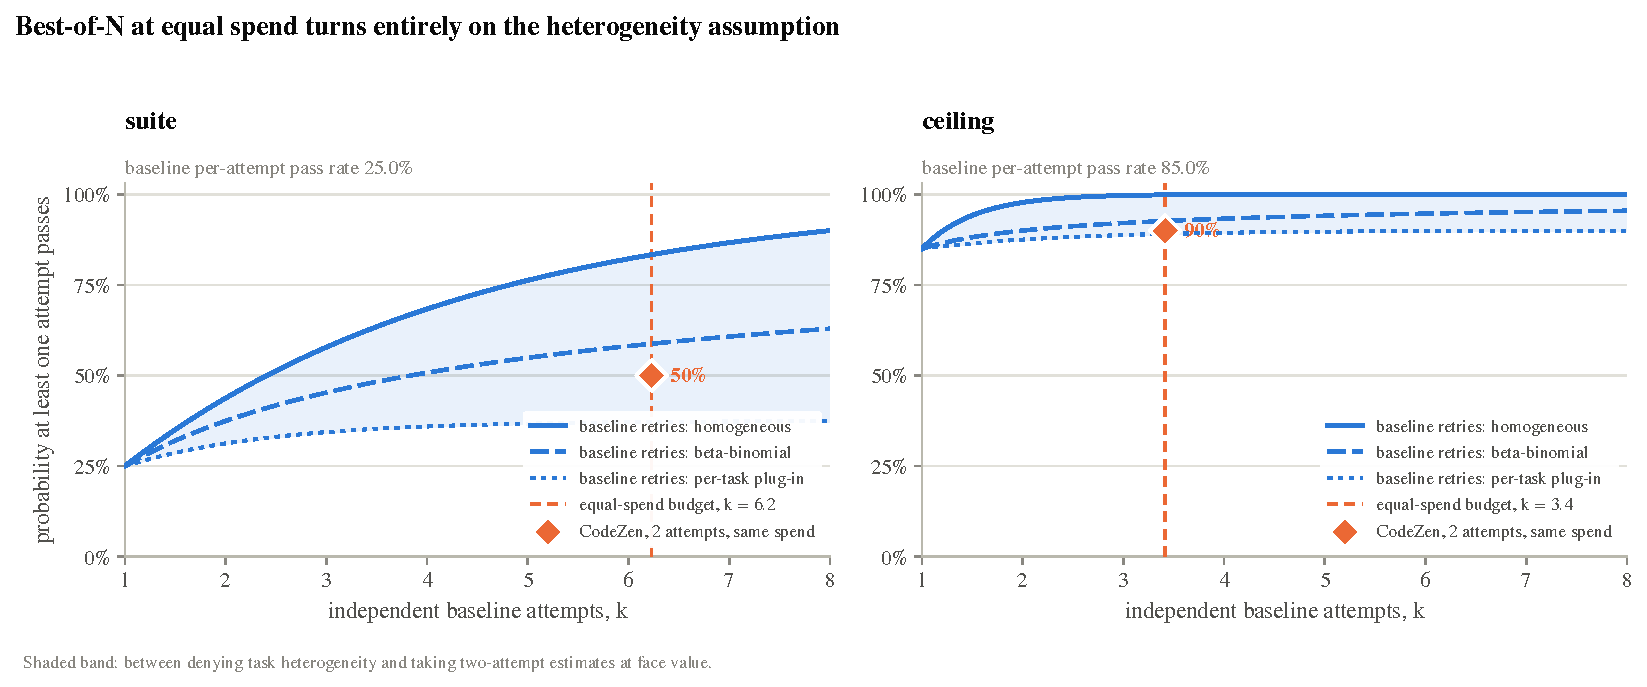
\includegraphics[width=\linewidth]{figures/x09-best-of-n.pdf}
\caption{Best-of-$N$ curves under the three estimators, with the equal-spend budget marked.
CodeZen's measured result sits \emph{inside} the band on the \emph{suite} population.}
\label{fig:bestofn}
\end{figure}

\begin{finding}{Bounded, not settled}
On the \emph{suite} population, at 6.2 baseline attempts for the price of CodeZen's two, the
retry strategy reaches somewhere between \textbf{37\,\% and 83\,\%} depending on how task
heterogeneity is modelled, against CodeZen's measured \textbf{50\,\%}. The homogeneous model
favours retries by 33 points, the beta-binomial by 8.6, and the plug-in model favours
\emph{CodeZen} by 12.8. The sign changes with the estimator, so ``repeated sampling strictly
dominates'' is \textbf{not established}. It remains the most plausible reading --- two of three
estimators favour retries, and the dissenting one has the clearest upward bias in its
assumptions --- but ``plausible'' is the correct word.

On the \emph{ceiling} population no estimator is needed: baseline already passes 89.5\,\% of
graded trials, so extra attempts buy almost nothing and the overhead is a pure loss rather
than a trade. All three estimators put baseline retries at or above CodeZen's 90\,\%.

None of this is a measurement. \textbf{Nobody has run baseline at $3\times$ the attempts and
compared.} That experiment needs no new infrastructure, is the comparison an operator actually
faces, and would replace a three-estimator range with a number. It is the highest-value cheap
experiment left.
\end{finding}

\section{What this supports, what it does not, and what binds it}
\label{sec:limits}

\begin{finding}{Supported}
\begin{enumerate}[nosep]
\item CodeZen costs $1.71\times$ baseline on work that completes and $3.11\times$ on work that
      does not, for $0.96$--$1.00\times$ the partial credit. Significant on two independent
      populations, with delegation as the measured mechanism.
\item Process converts into censoring risk: $1.90\times$ budget consumption, 25\,\% of CodeZen
      trials killed by the clock against 9.6\,\% for baseline and SDD.
\item Methodology can regress a solved task, and can make a solved task less reliable.
\item 71\,\% of toolkit trials invoked no toolkit skill. Availability was total.
\item Human-expert difficulty does not predict agent difficulty ($\rho = -0.078$, $p = 0.70$).
\item The one-trial screening rule is unreliable in both directions, and all three screens in
      this sequence overshot.
\item The censoring convention is decision-relevant, not cosmetic, and 7 of 23 kills discarded
      a workspace that already scored 1.0.
\end{enumerate}
\end{finding}

\begin{finding}{Not supported}
\begin{enumerate}[nosep]
\item Any claim about which configuration produces better outcomes. 18 of 26 tasks are
      concordant and effective $n$ is 1--5.
\item That SDD's partial-credit shortfall is real rather than noise ($p = 0.125$ at $n = 10$),
      although it appears at the same magnitude on both populations.
\item Any causal reading of ``skill-invoking trials mostly failed''. Selection and effect are
      inseparable here.
\item That retries beat process at equal spend. The sign changes with the estimator.
\item Anything about the regime methodologies are written for: multi-session work with
      ambiguous requirements and a human in the loop.
\end{enumerate}
\end{finding}

\noindent\textbf{The five confounds that actually bind.}

\begin{enumerate}
\item \textbf{The measured population is not the target population.} Terminal-Bench tasks are
      single-session, self-contained and fully specified --- the regime where a specification
      process has least to add. No result here transfers to the regime where it might have
      most. Evaluating such a process needs task populations in which ambiguity and
      coordination are genuine sources of difficulty \citep{ribeiro2020ambiguity}, which is a
      task-construction problem --- and construction defects are not hypothetical
      \citep{openai2026signal}.
\item \textbf{The condition is a repository, not a methodology text.} Toolkits deploy in full,
      so \code{docs/}, \code{tools/} and \code{standards/} land beside the task. That is the
      ecologically valid unit, but a broader one than ``the methodology''.
\item \textbf{\code{codezen-viable} is a curated four-skill subset} of an eleven-skill toolkit.
      Nothing here speaks to the full toolkit.
\item \textbf{Method availability, not enforcement.} The agent was never instructed to follow
      the repository's process, and mostly did not.
\item \textbf{Concurrency inflates the clock.} Nine trials ran at a time on one host, so
      wall-clock and the derived budget share carry contention; cost and token metrics do not.
      Contention is symmetric within a task, so the paired comparisons survive, but the
      absolute budget percentages are inflated.
\end{enumerate}

\begin{finding}{The general form of the finding}
The result is not that these two toolkits are badly built. It is that a fixed process applied
unconditionally is the wrong shape of thing for an agent under a bounded budget. Process
research already holds that a standardised process should be tailored to its context
\citep{xu2007tailoring}; the test-time compute literature already holds that the best use of
an extra unit of compute depends on the instance \citep{snell2024scaling}; and cost-aware
agent evaluation already holds that resource efficiency belongs among the dependent variables
\citep{liu2026costbench}. Read together with the evidence above:

\smallskip
\emph{Autonomous coding methodology is better treated as an adaptive resource-allocation
policy than as a universally beneficial fixed process.}
\smallskip

This experiment supplies the instance. The same review machinery that is defensible while the
artefact is still failing becomes harmful once it already passes, because continued process
consumes the one resource the trial needs in order to terminate --- and in seven trials it
converted finished work into a censored observation.
\end{finding}

\clearpage
\section{What to change}
\label{sec:changes}

\begin{figure}[htbp]
\centering
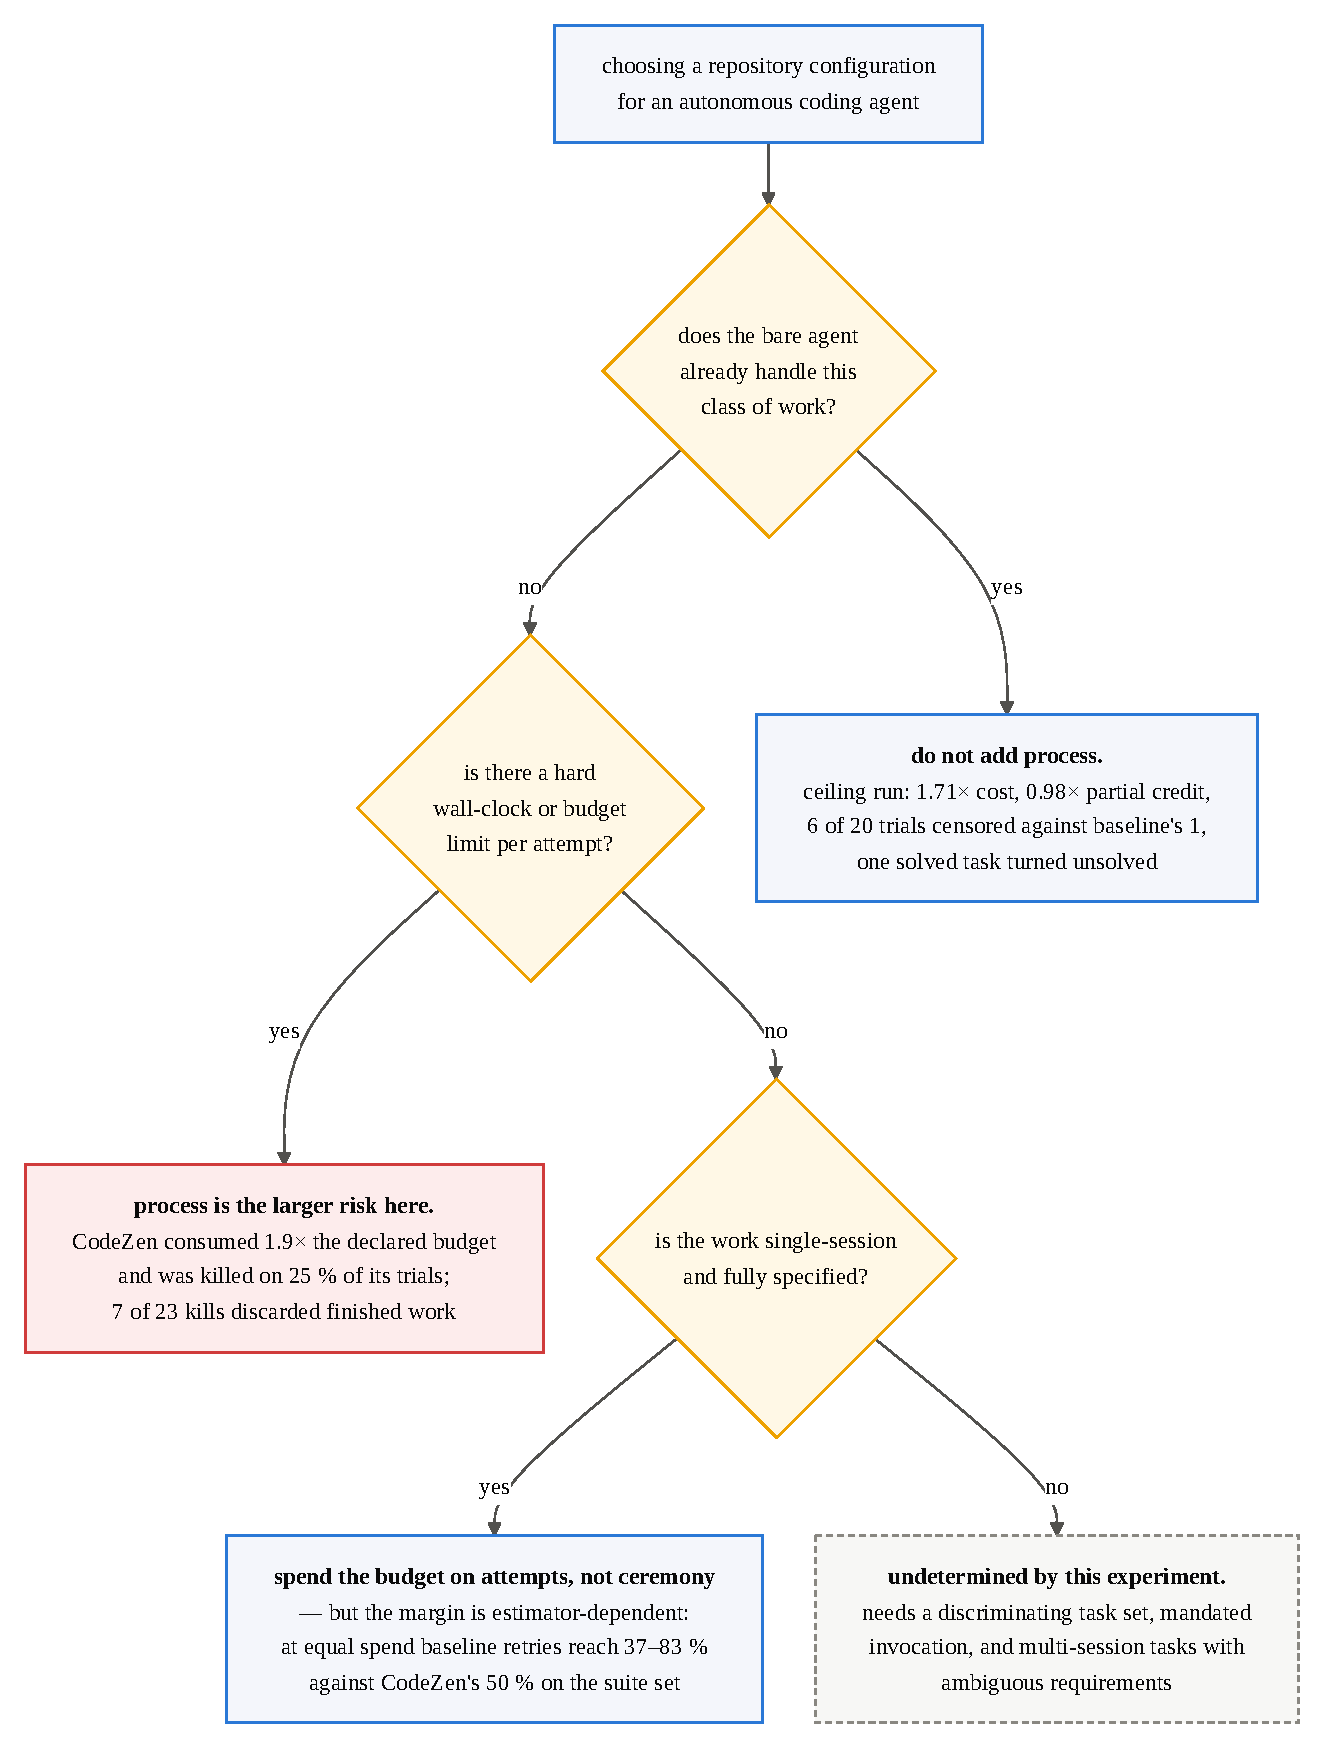
\includegraphics[width=0.60\linewidth]{diagrams/d07-operator-decision.pdf}
\caption{The decision this measurement supports, with the evidence attached to each branch.
One branch is marked undetermined on purpose: the experiment does not reach the regime
methodologies are written for.}
\label{fig:decision}
\end{figure}


\begin{center}\small
\begin{tabular}{@{}p{5.4cm}p{10.0cm}@{}}
\toprule
Change & Why \\
\midrule
\textbf{Grade the workspace at the moment of the kill} &
7 of 23 kills scored 1.0 anyway. Turns censoring from a lost observation into a measured one,
removes the convention choice, repairs the long end of the length analysis. Costs no model
tokens. Do this first \\
\addlinespace
\textbf{Screen on baseline pass \emph{rate}, not one outcome} &
Keep a task when 1 or 2 of 3 baseline trials pass. The one-trial rule cannot distinguish
``always fails'' from ``sometimes fails'', and only the second discriminates. Roughly
$2\times$ the screen's cost, and the only change that materially improves outcome power \\
\addlinespace
\textbf{Randomise invocation} --- mandate the process in half the trials &
Makes ``enforcement'' a manipulated variable, breaks the selection/effect confound, and answers
the question most people actually mean when they ask whether a methodology works \\
\addlinespace
\textbf{Run the equal-budget retry comparison} &
One methodology trial against $2k$ baseline attempts, same tasks, same money. Replaces
\S\ref{sec:bestofn}'s range with a measurement \\
\addlinespace
\textbf{Gate procedural skills on state and on time remaining} &
An agent should not open a delegated review when the tests are already green, or with a small
fraction of its budget left. This is an agent-design change, not a benchmark one, and it is the
directly actionable output of \S\ref{sec:trap} \\
\bottomrule
\end{tabular}
\end{center}

\clearpage
\section{Provenance, and where the numbers come from}

This report consolidates two per-run analyses, one cross-run synthesis, and an independent
critical review of all three contributed by Antigravity (Google DeepMind). Every quantity was
recomputed from the exported per-trial tables by \code{whitepaper/scripts/}\allowbreak
\code{verify\_numbers.py}, independently of the source documents. That recomputation surfaced
nine disagreements; three of them change something a reader would act on, and are recorded
here. The remaining six, the full divergence record, every censored trial, the complete
correlation matrix and the per-task tables are in \code{main.pdf}.

\begin{center}\footnotesize
\begin{tabular}{@{}p{3.0cm}p{3.4cm}p{3.4cm}p{4.6cm}@{}}
\toprule
Quantity & Source reading & Independent review & Recomputed, and what follows \\
\midrule
Best-of-$N$ at equal spend &
open question, not computed &
57.8\,\% vs 36.0\,\%, ``strictly dominates'' &
Estimator-dependent, \textbf{37--83\,\%} against 50\,\% (\S\ref{sec:bestofn}). Downgraded to
``most plausible reading, not established'' \\
\addlinespace
\task{headless-terminal} baseline duration and cost &
not quoted &
253.4\,s and 648.9\,s, \$0.48 and \$0.78; ``exits on green tests'' &
\textbf{144.5\,s and 114.1\,s, \$0.27 and \$0.20}, with \textbf{zero} recognised test runs on
either attempt. The ratio is $8.1\times$ and $14.1\times$, not $3.6\times$ and $5.2\times$.
The trap is real and larger than reported \\
\addlinespace
\task{torch-pipeline-} \task{parallelism} baseline reliability &
``passes inside 34\,\% of budget'' &
``succeeded easily inside 34\,\% of the budget''; cites 1{,}175\,s &
Passes \textbf{one of two} attempts at 29\,\% of budget; the other failed at 2 of 3. No
baseline attempt took 1{,}175\,s. The regression stands; ``easily'' does not \\
\bottomrule
\end{tabular}
\end{center}

\medskip
\noindent\textbf{Reproducibility.} Terminal-Bench 2.0 task suite pinned at \code{2fd12b88};
agent Claude Code on \code{claude-sonnet-5}; both toolkits frozen at Git SHAs recorded in
\code{config/sources.yaml}; runs executed 2026-08-31 and 2026-09-01 at 9-way concurrency on one
host. Per-trial tables are \code{results/analysis-\{suite,ceiling\}/data/trials.csv};
\code{cd whitepaper \&\& make} regenerates every figure, diagram and table from them and
recompiles both this report and the full paper.

\clearpage
\noindent\small\emph{Provenance of the reference list.} The literature set follows the review
memo in \code{data/schmierzettel.txt}. Entries whose bibliographic details could not be
confirmed first-hand --- chiefly the 2026 works --- are flagged by a \code{\% VERIFY} comment
above the entry in \code{references.bib}, and \code{data/citation-map.md} records every
placement together with three points where the memo's attribution appears to be wrong and what
was used instead. Verify those before circulating either document.\normalsize
\smallskip

\bibliographystyle{plainnat}
\bibliography{references}

\end{document}
